\chapter{Results}

The results were produced using atomic units, i.e $\hbar=e=m_e=4\pi\epsilon_0 = 1$, where $m_e$ and $e_0$ is the electron mass and vacuum permittivity respectively. This implies that all listed energies are given in Hartrees, i.e. scaled with $\hbar^2/m_ea_0^2$, and all lengths are given in Bohr radii, i.e. scaled with $a_0=4\pi\epsilon_0\hbar^2/m_e e^2$.


\section{Optimization Results}
\label{sec:optRes}

The optimization results listed in this section are estimated using a 30-particle two-dimensional quantum dot as reference system.

Profiling the code revealed that $\sim99\%$ of the run time was spent diffusing the particles, that is, spent in the function \verb+QMC::diffuse_walker+. Variational Monte-Carlo (VMC), Diffusion Monte-Carlo (DMC), and Adaptive Stochastic Gradient Descent (ASGD) all rely heavily on the diffusion of particles, hence the parts of the code which do not involve diffusion walkers were neglected in the optimization process; it is a waste of time to optimize something which accounts for less than one percent of the run time.  

The profiling tool of choice was \textit{KCacheGrind}, which is available for free at the Ubuntu Software Center. KCacheGrind lists relative time spent in functions graphically in blocks whose sizes are proportional to the time spent inside the functions, much like standard hard drive listing software does with files and file sizes.

Optimizations discussed in Chapter \ref{ch:optAndGen} which are not mentioned in the following sections were considered standard implementations, and were thus implemented prior to the optimization process.

\subsubsection{Storing the Slater matrix}

This optimization is described in detail in Section \ref{sec:storeSlater}. In addition to storing the Slater matrix, the calculation of $\mathbf{\tilde I}$ from the inverse updating algorithm in Eq.~(\ref{eq:Itilde}) was taken outside of the main loops.

The percentages listed in the following table represent the ratio between the total time spent inside the given function and the total run time. 

\begin{tabular}{ll}
 \verb+Orbitals::phi+ & \\
 \hline\hline
 Relative run time used prior to optimization & 80.88\% \\
 Relative run time used after optimization    & 8.2\% \\
 \hline
 Relative function speedup                   & 9.86
\end{tabular}

The speedup comes not as a result of optimizations within the function itself, but rather as a result of far less calls to the function. If $\mathbf{\tilde I}$ was calculated outside of the main loops in the first place, the speedup would be far less significant. 


\subsubsection{Optimized Jastrow gradient}

The optimization described in this section is discussed in detail in Section \ref{sec:optJastGrad}.

The percentages listed in the following table represent the ratio between the total time spent inside the given functions and the total run time. 

\begin{tabular}{ll}
 \verb+Jastrow::get_grad+ \& \verb+Jastrow::calc_dJ+ & \\
 \hline\hline
 Relative run time used prior to optimization & 40\% \\
 Relative run time used after optimization    & 5.24\% \\
 \hline
 Relative function speedup                   & 7.63
\end{tabular}

Exploiting the symmetries of the Padé Jastrow gradient, in addition to calculating the new gradient based on the old, are in other words extremely efficient. Keep in mind that these results are for a high number of particles. For two particles, this optimization would not matter at all.

\subsubsection{Storing the orbital derivatives}

This optimization is covered in detail in Section \ref{sec:storeSlater}. Much like for the Slater matrix, the optimization in this case comes from the fact that the function itself is called fewer times, rather than being faster.

The percentages listed in the following table represent the ratio between the total time spent inside the given function and the total run time. 


\begin{tabular}{ll}
 \verb+Orbitals.dell_phi+ & \\
 \hline\hline
 Relative run time used prior to optimization & 56.27\% \\
 Relative run time used after optimization    & 7.31\% \\
 \hline
 Relative function speedup                   & 7.70
\end{tabular}


\subsubsection{Storing quantum number independent terms}

This optimization is covered in detail in Section \ref{sec:optSPWFqnumIndie}. The result of the optimization is a reduction in the number of exponential function calls, which means a more efficient calculation of single-paticle states, their gradients and Laplacians.

The percentages listed in the following table represent the ratio between the total time spent inside the given functions and the total run time. 

\begin{tabular}{ll}
 \verb+Orbitals::phi+ \& \verb+Orbitals::dell_phi+ & \\
 \hline\hline
 Relative run time used prior to optimization & 5.85\% \\
 Relative run time used after optimization    & 0.13\% \\
 \hline
 Relative function speedup                   & ~45
\end{tabular}

This result is not surprisingly equal to $15\cdot 3$, since a 30-particle quantum dot has $15$ unique quantum numbers. One set is used by the orbitals, and two by their gradients (the Laplacian is not a part of the diffusion). Prior to this optimization, $45$ exponential calls were needed to fill a row in the Slater matrix and the derivative matrix; this has been reduced to one.

\subsubsection{Overall optimization and final scaling}

Combining all the optimizations listed in this section, the final run time was reduced to $5\%$ of the original. The final scaling is presented in Figure \ref{fig:scaling}.

\begin{figure}[h]
 \begin{center}
  \subfigure{\includegraphics[scale=0.35]{../Graphics/scaling.png}}
  \subfigure{\includegraphics[scale=0.35]{../Graphics/scaling_loglog.png}} \\
  \caption{Scaling of the code with respect to the number of particles $N$ based on VMC calculations with $10^6$ cycles with $10^5$ thermalization steps run on eight processors. The figures are split into a low $N$ region and a high $N$ region. Only two-dimensional quantum dots and atoms are displayed in the high $N$ figure. The figures to the right contain the same data as the figures to the left, however, displayed using logarithmic axes. As expected, the two-dimensional quantum dots (denoted Qdots 2D) are lowest on run time and the homonuclear diatomic molecules are highest (denoted Molecules). The logarithmic figures clearly show a linear trend, implying a underlying power law.}
  \label{fig:scaling}
 \end{center}
\end{figure}

The following power laws are deduced based on linear regression of the above figures for $N > 2$

\begin{tabular}{l|c}
System & Scaling \\
\hline
Two dimensional quantum dots & $N^{2.1038}$ \\
Three dimensional quantum dots & $N^{2.1008}$ \\
Atoms & $N^{1.8119}$ \\
Homonuclear diatomic molecules & $N^{1.8437}$ \\ 
\end{tabular}


As the number of particles $N$ increases, the scaling with respect to the number of spatial dimensions $d$ becomes negligible compared to the scaling with $N$, rendering two-dimensional quantum dots and atoms similar in run time. This is expected since there are far more matrices in the code of dimensions $N\times N$ than $N \times d$. 

The Jastrow factor, inverse updating, etc., all involve the same computations for all systems, hence the reason why the atomic systems scale better than the quantum dots has to originate from the efficiency of the single-paticle wave functions. Consider for example the third single-paticle wave function for the hydrogen-like orbitals (omitting exponential factors):

\begin{equation}
 \phi_3 = x.
\end{equation}

The corresponding expression for a two-dimensional quantum dot is

\begin{equation}
  \phi_3 = 2k^2y^2 - 1.
\end{equation}

It is obvious that the orbital for quantum dots contains a higher computational cost for the processor than the one for atoms. Comparing the expressions listed for quantum dots in Appendix \ref{appendix:SymPyHO3D} and Appendix \ref{appendix:SymPyHO} with those for atoms in Appendix \ref{appendix:SymPyHydro}, it is apparent that this trend is consistent.

The fact that the difference in the cost of the single-paticle wave functions govern the scaling demonstrates the efficiency in the general framework. Moreover, having the molecular system scaling almost identically to the atomic one demonstrates the efficiency of the system's implementation. 

Both Variational Monte-Carlo and Adaptive Stochastic Gradient Descent scale linearly with the number of processors, due to the fact that the processes do not require any communication besides adding the final results. Diffusion Monte-Carlo, on the other hand, is parallelized by spreading the original walker population across multiple nodes. Depending on whether some nodes have more deaths or newborns than others, there is a high communication cost. What is seen in practice, however, is that as long as the average number of walkers per node does not go below $\sim250$, the scaling is approximately linear. 





\clearpage
\section{The Non-interacting Case}

In the case of non-interacting particles, that is, the case with no electron-electron interaction, the trial wave function represents the exact wave function both in the case of quantum dots and atoms. For molecules and the double-well quantum dot, the additional requirement that $R\to\infty$ should also be applied, where $R$ is the distance between the atoms in the case of molecules, and the distance between the well centers in the case of the quantum dot. All of the presented systems are covered in detail in Chapter \ref{ch:modelledSystems}.

Exact solutions serve as a powerful guide, since results can be benchmarked against these, that is, the code can be validated. In the non-interacting case, Adaptive Stochastic Gradient Descent (ASGD) should always provide a variational parameter equal to unity, i.e. $\alpha=1$. Variational Monte-Carlo (VMC) and Diffusion Monte-Carlo (DMC) should reproduce the exact solutions from Eq.~(\ref{eq:qdotsE0}) in the case of quantum dots and Eq.~(\ref{eq:atomsE0}) in the case of atomic systems to machine precision. 

In Table \ref{tab:res_valid_qdots}, validation runs for the three lowest lying closed-shell quantum dots are run for both two and three dimensions. Figure \ref{fig:ASGD_nonint} shows ASGD finding the exact minimum. Table \ref{tab:res_valid_atoms} shows similar results for atoms. As required, the closed form energies are reproduced to machine precision.

The double-well quantum dots results reproduce the non-interactive energies when the wells are placed far enough apart. This is demonstrated in Table \ref{tab:res_valid_qdots_doublewell}. A separation equal to $R = 20$ was sufficient. For molecules, on the other hand, the atomic nuclei interaction is very strong, implying the need of a greater separation of the atoms than what was needed for the wells. Table \ref{tab:res_valid_molecules} shows this effect; the convergence is nice for $\mathrm{H_2}$, however, for the heavier molecules, where the atomic nuclei interaction is higher, the convergence to the non-interacting limit is slower.

DMC should in the case of an exact wave function be perfectly stable. The trial energy should equal the ground state energy through all time steps and zero fluctuations in the number of walkers should occur. This trend is shown for the Neon atom in figure \ref{fig:DMC_neon_nonint}.

A final non-interacting case is run for DMC without the exact wave function. As discussed in Chapter \ref{ch:QMC}, DMC should result in a better estimate of the ground state energy than VMC in the case of a trial wave function which is different from the exact ground state. A test case is presented in figure \ref{fig:DMC_nonExactWF}.

\setlength{\tabcolsep}{0.3cm}
\begin{table}[h]
\begin{center}
\begin{tabular}{c|cccccc||cccccc}
 & & & 2D & & & & & & & 3D \\
\hline
  $\omega$   & N & $\mathrm{E_{VMC}}$ & $\mathrm{E_{DMC}}$ & $\alpha$ & $E_0$ & \qquad  & \qquad &  N   & $\mathrm{E_{VMC}}$ & $\mathrm{E_{DMC}}$ & $\alpha$ & $E_0$ \\
\hline
 0.5 &   2   &   1.0    &   1.0    &   1.0    & 1  & \qquad & \qquad & 2     &   3.0   &   3.0    &   1.0    & 3 \\
 1.0 &       &   2.0    &   2.0    &   1.0    & 2  & \qquad & \qquad &       &   1.5   &   1.5    &   1.0    & 1.5 \\
 0.5 &   6   &   5.0    &   5.0    &   1.0    & 5  & \qquad & \qquad &  8    &   18.0  &   18.0   &   1.0    & 18 \\
 1.0 &       &   10.0   &   10.0   &   1.0    & 10 & \qquad & \qquad &       &  9.0    &   9.0    &   1.0    & 9 \\
 0.5 &   12  &   14.0   &   14.0   &   1.0    & 14 & \qquad & \qquad & 20    &  60.0   &   60.0   &   1.0    & 60 \\
 1.0 &       &   28.0   &   28.0   &   1.0    & 28 & \qquad & \qquad &       &  30.0   &   30.0   &   1.0    & 30 \\
\end{tabular}
\caption{Validation results for $N$-particle quantum dots with no Coulomb interaction and frequency $\omega$. The left-hand side shows the results for two dimensions, while the results for three dimensions are listed on the right-hand side. The last column for each dimension lists the exact energies $E_0$ calculated from Eq.~(\ref{eq:qdotsE0}). The exact solution to $\alpha$ is unity. As required, all methods reproduce the exact results. The variance is zero to machine precision for all listed results.}
\label{tab:res_valid_qdots}
\end{center}
\end{table}
\setlength{\tabcolsep}{6pt}

\setlength{\tabcolsep}{0.8cm}
\begin{table}[h]
\begin{center}
\begin{tabular}{cc|cccc}
  $\omega$   & N & $\mathrm{E_{VMC}}$ & $\mathrm{E_{DMC}}$ & $\alpha$ & $E_0(R\to\infty)$ \\
\hline
  0.5  &       &   4.0   & 4.0   &   1.0    & 4   \\
  1    &   4   &   2.0   & 2.0   &   1.0    & 2   \\
  0.5  &       &   20.0  & 20.0  &   1.0    & 20  \\
  1    &   12  &   10.0  & 10.0  &   1.0    & 10  \\
  0.5  &       &   28.0  & 28.0  &   1.0    & 28   \\
  1    &   24  &   56.0  & 56.0  &   1.0    & 56   \\
\end{tabular}
\caption{Validation results for $N$-particle double-well quantum dots with no Coulomb interaction and frequency $\omega$. The exact energy $E_0$, calculated from  Eq.~(\ref{eq:qdotsE0}), is listed in the last column. The calculations are performed with the wells separated at a distance $R=20$ in the $x$-direction. The exact solution to $\alpha$ is unity. As for the single-well quantum dots in Table \ref{tab:res_valid_qdots}, all methods reproduce the exact solution. The variance is zero to machine precision for all listed results. }
\label{tab:res_valid_qdots_doublewell}
\end{center}
\end{table}
\setlength{\tabcolsep}{6pt}

\setlength{\tabcolsep}{0.8cm}
\begin{table}
\begin{center}
\begin{tabular}{cc|cccc}
 Atom &   N     & $\mathrm{E_{VMC}}$ & $\mathrm{E_{DMC}}$ & $\alpha$ & $E_0$\\
\hline
 $\mathrm{He}$ &   2     &   -4.0   &   -4.0   &   1.0  & -4  \\
 $\mathrm{Be}$ &   4     &  -20.0   &  -20.0   &   1.0  & -20 \\
 $\mathrm{Ne}$ &   10    &  -200.0  &  -200.0  &   1.0  & -200\\
\end{tabular}
\caption{Validation results for different atoms consisting of $N$ electrons with no electron-electron Coulomb interaction. The exact energies $E_0$ are calculated from Eq.~(\ref{eq:atomsE0}). The exact solution of the variational parameter $\alpha$ is unity. As required, all methods reproduce the exact solutions. The variance is zero to machine precision for all listed results.}
\label{tab:res_valid_atoms}
\end{center}
\end{table}
\setlength{\tabcolsep}{6pt}

\setlength{\tabcolsep}{0.6cm}
\begin{table}
\begin{center}
\begin{tabular}{cc|cccc}
 Molecule &   N     & $R$ & $\mathrm{E_{VMC}}$ & $\mathrm{E_{DMC}}$ & $E_0(R\to\infty)$\\
\hline
 $\mathrm{H}_2$  & 2     & 10  &   -0.847    &  -0.9968    & -1  \\
   &       & 100  &  -0.979    &  -0.995  &  \\
   &       & 325   &  -1.000    &  -1.000  &  \\
 $\mathrm{Be}_2$  & 8     & 10  &  -41.596     &  -41.608   & -40 \\
  &        & 100 &  -40.298     &  -40.231   &     \\
   &       & 325 &  -40.123     &  -40.112   &     \\
 $\mathrm{Ne}_2$ &  20    & 10  &  -409.999    &  -410.010  & -400\\
  &        & 100 &  -401.390    &  -401.049  &     \\
  &        & 325 &  -           &  -         &     \\
\end{tabular}
\caption{Validation results for homonuclear diatomic molecules separated at a distance $R$ with no electron-electron interaction. The last column lists the exact energies $E_0$ calculated from Eq.~(\ref{eq:atomsE0}) for $R\to\infty$. Choosing $R$ too high results in a singular Slater determinant due to finite machine precision. This happens already for $R=325$ in the case of  $\mathrm{Ne}_2$. It is apparent that increasing $R$ brings the solutions closer to the exact energy. The statistical error is skipped.}
\label{tab:res_valid_molecules}
\end{center}
\end{table}
\setlength{\tabcolsep}{6pt}


\begin{figure}[h]
 \begin{center}
  \subfigure{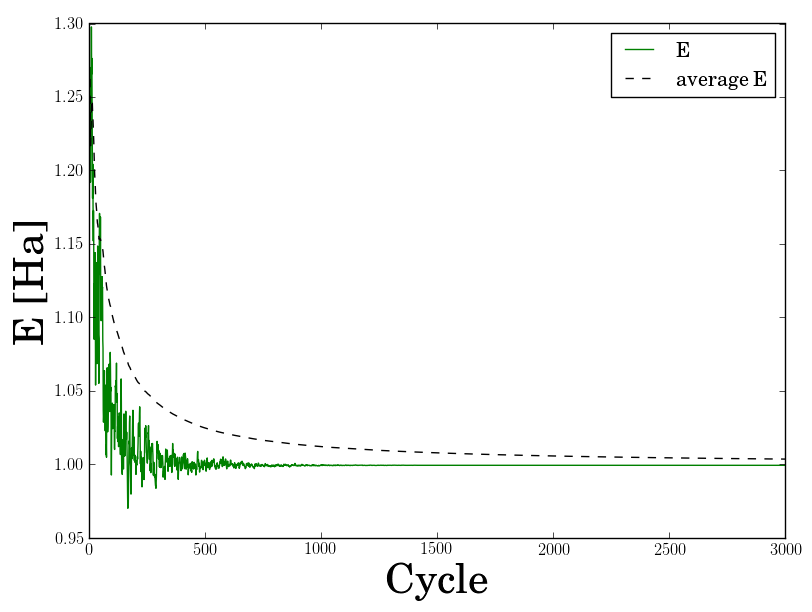
\includegraphics[scale=0.37]{../Graphics/ASGD_nonint_E.png}}
  \subfigure{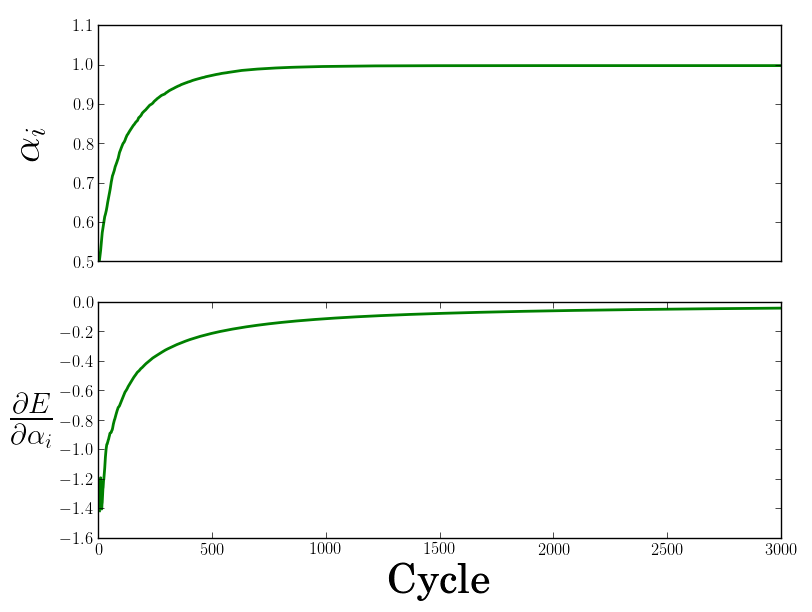
\includegraphics[scale=0.37]{../Graphics/ASGD_nonint.png}} 
  \caption{Adaptive Stochastic Gradient Descent (ASGD) results for a two-particle two-dimensional quantum dot with frequency $\omega=0.5$ and no electron-electron interaction. The exact energy $E_0=1$ is reached after approximately 1000 cycles, where the variational parameter $\alpha$ has converged close to unity. Due to enormous fluctuations the variational derivative is plotted as an accumulated average. The gradient is approximately zero after ~1000 cycles, in agreement with the behavior of the energy. The variational principle described in Section \ref{sec:selectingOptVarPar} is governing the trend of the energy convergence, however, a lot of statistical noise is present in the first 1000 cycles due to a high variance and a small number of samples.}
  \label{fig:ASGD_nonint}
 \end{center}
\end{figure}



\begin{figure}[h]
 \begin{center}
  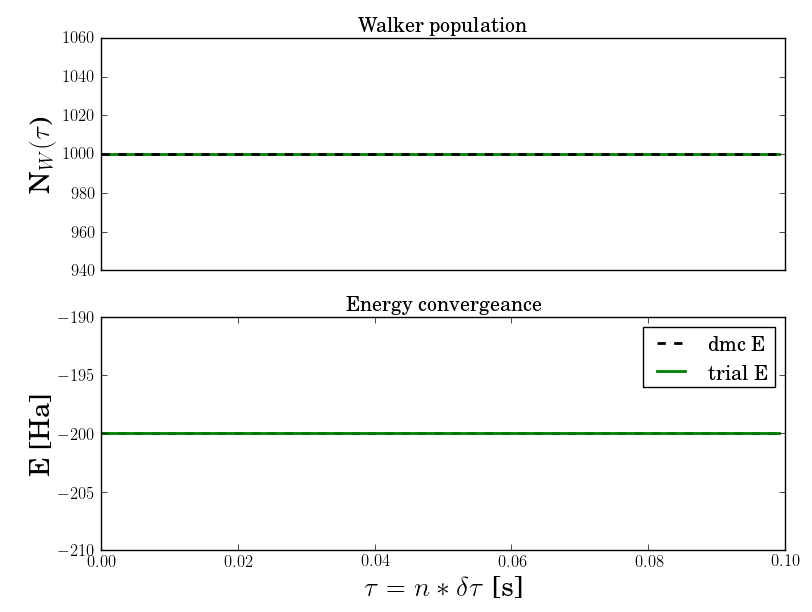
\includegraphics[scale=0.5]{../Graphics/DMC_neon_valid.png}
  \caption{Illustration of the Diffusion Monte-Carlo (DMC) energy convergence for the Neon atom listed in Table \ref{tab:res_valid_atoms}. The trial energy is fixed at the exact ground state energy as required. The number of walkers are constant, implying an approximately zero variance in the samples.}
  \label{fig:DMC_neon_nonint}
 \end{center}
\end{figure}

\begin{figure}[h]
 \begin{center}
  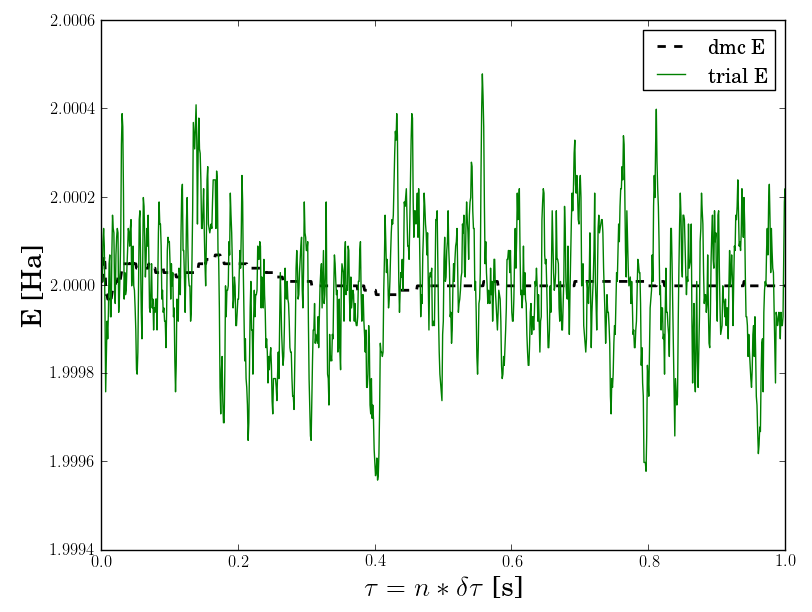
\includegraphics[scale=0.5]{../Graphics/DMC_notExactWF.png}
  \caption{Illustration of the Diffusion Monte-Carlo (DMC) energy convergence for a two-particle two-dimensional quantum dot with frequency $\omega=1$. The calculations are done with a variational parameter $\alpha=0.75$, where as the exact wave function is given for $\alpha=1$. Unlike the case with the exact wave function presented in figure \ref{fig:DMC_neon_nonint}, the trial energy oscillates around the exact value $E_0 = 2.0$. The final result reveals a DMC energy of $2.00000(2)$, where the original Variational Monte-Carlo (VMC) energy was $2.0042(3)$. This illustrates the power of DMC contra VMC in the interesting cases where the exact wave function is unknown. The calculation was done using $10000$ random walkers.}
  \label{fig:DMC_nonExactWF}
 \end{center}
\end{figure}
\clearpage
\section{Quantum Dots}

The focus regarding quantum dots has been on studying the distribution of electrons as a function of the level of confinement. In addition, ground state energies are provided and compared to other many-body methods to demonstrate the efficiency and precision of Variational Monte-Carlo (VMC) and Diffusion Monte-Carlo (DMC). In the case of two-dimensional quantum dots, there are multiple published results, however, for three dimensions this is not the case. An introduction to quantum dots is given in Section \ref{sec:modelQDots}. 

The double-well quantum dot has not been a focus in this thesis, however, some simple results are provided to demonstrate the flexibility of the code.

\subsection{Ground State Energies}

\subsubsection{Two-dimensional quantum dots}

Table \ref{tab:QDotsResultsAll} presents the calculated ground state energies for two-dimensional quantum dots in addition to corresponding results from methods such as Similarity Renormalization Group theory (SRG), Coupled Cluster Singles and Doubles (CCSD) and Full Configuration Interaction (FCI). In addition, some previously published DMC results are supplied. The references are listed in the table caption.

In light of the variational nature of DMC and VMC, the results show that DMC provides a more precise estimate for the ground state energy than VMC, both in terms of lower energies and lower errors. The exact energy in the case of two electrons with $\omega=1$ has been calculated in Ref. \cite{taut} and is $E_0 = 3$, which is in excellent agreement with the presented results.

The statistical errors in the DMC energies calculated in this thesis are lower than those provided in Ref. \cite{MagnusArticle}. This may only be due to the fact that the calculations in this thesis have been run on a super computer. Running smaller simulations on fewer processors result in larger errors. Both the implementations successfully agree with the FCI result for two particles, which strongly indicates that the disagreements in results are a result of systematic errors.    

In the case of two particles, DMC and FCI agree up to five decimals, which leads to the conclusion that DMC indeed is a very precise method. The SRG method is not variational in the sense that it can undershoot the exact energy. The DMC result should thus not be read as less precise in the cases where SRG provides a lower energy estimate. Diffusion Monte-Carlo and SRG are in excellent agreement for a large number of particles compared to FCI and CCSD, which drift away from the DMC results as their basis sizes shrink. 

For high frequencies, the VMC energy is higher than the CCSD energy. The fact that both the methods are variational implies that CCSD performs better than VMC in this frequency range. However, looking at the results the lower frequency range, it is clear that VMC performs better than CCSD. This is due to the fact that CCSD struggles with convergence as the correlations within the system increase, indicated by the decrease in number of shells used to perform the calculations.

The DMC energy is overall smaller than the CCSD energy, which, due to the variational nature of the methods, implies that DMC performs better than CCSD. Nevertheless, the results for $56$ particles are in excellent agreement. 

\setlength{\tabcolsep}{5pt}
\begin{table}
\begin{center}
\begin{tabular}{cc|rrrrrr}
    N     & $\omega$ & $\mathrm{E_{VMC}}$ & $\mathrm{E_{DMC}}$ & $E_\mathrm{ref}^{(a)}$& $E_\mathrm{ref}^{(b)}$ & $E_\mathrm{ref}^{(c)}$ & $E_\mathrm{ref}^{(d)}$\\
\hline\hline
\multicolumn{8}{c}{} \\
    2     &   0.01   & 0.07406(5)  & 0.073839(2)  & -		& -			& 0.0738 \{23\} & 0.07383505 \{19\}\\
          &   0.1    & 0.44130(5)  & 0.44079(1)   & - 		& - 			& 0.4408 \{23\} & 0.44079191 \{19\}\\
          &   0.28   & 1.02215(5)  & 1.02164(1)   & -		&0.99263 \{19\} 	& 1.0217 \{23\}  & 1.0216441 \{19\}\\
          &   0.5    & 1.66021(5)  & 1.65977(1)   & 1.65975(2)&1.643871 \{19\}	& 1.6599 \{23\}  & 1.6597723 \{19\}\\
          &   1.0    & 3.00030(5)  & 3.00000(1)   & 3.00000(3)&2.9902683 \{19\}	& 3.0002 \{23\}  & 3.0000001 \{19\}\\
\cline{2-8}
\multicolumn{8}{c}{} \\
    6     &   0.1    &  3.5690(3)  &  3.55385(5)  & -		&3.49991 \{18\} 	& 3.5805 \{22\}  & 3.551776 \{9\}\\
          &   0.28   &  7.6216(4)  &  7.60019(6)  & 7.6001(1) &7.56972 \{18\} 	& 7.6254 \{22\}  & 7.599579 \{6\}\\
          &   0.5    & 11.8103(4)  & 11.78484(6)  & 11.7888(2)&11.76228 \{18\}	& 11.8055 \{22\} & 11.785915 \{6\}\\
          &   1.0    & 20.1902(4)  & 20.15932(8)  & 20.1597(2)&20.14393 \{18\}	& 20.1734 \{22\} & 20.160472 \{8\}\\
\cline{2-8}
\multicolumn{8}{c}{} \\
    12    &   0.1    & 12.3162(5)  & 12.26984(8)  & - 		&12.2253 \{17\} 	& 12.3497 \{21\} & 12.850344 \{3\}\\
          &   0.28   & 25.7015(6)  & 25.63577(9)  & - 		&25.61084 \{17\} 	& 25.7095 \{21\} & 26.482570 \{2\}\\
          &   0.5    & 39.2343(6)  & 39.1596(1)   & 39.159(1) &39.13899 \{17\}	& 39.2194 \{21\} & 39.922693 \{2\}\\
          &   1.0    & 65.7905(7)  & 65.7001(1)   & 65.700(1) &65.68304 \{17\}	& 65.7399 \{21\} & 66.076116 \{3\}\\
\cline{2-8}
\multicolumn{8}{c}{} \\
    20    &   0.1    &  30.0729(8)  &  29.9779(1) & -		&29.95345 \{16\}	& 30.2700 \{8\} & 34.204867 \{1\}\\
          &   0.28   &  62.0543(8)  &  61.9268(1) & 61.922(2) &61.91368 \{16\}	& 62.0676 \{20\} & 67.767987 \{1\}\\
          &   0.5    &  94.0236(9)  &  93.8752(1) & 93.867(3) &93.86145 \{16\}	& 93.9889 \{20\} & 100.93607 \{1\}\\
          &   1.0    & 156.062(1)   & 155.8822(1) & 155.868(6)&155.8665 \{16\}	& 155.9569 \{20\}& 164.61280 \{1\}\\
\cline{2-8}
\multicolumn{8}{c}{} \\
    30    &   0.1    &  60.584(1)  &  60.4205(2)  & -		&60.43000 \{15\}	&  61.3827 \{9\}& -\\
          &   0.28   & 124.181(1)  & 123.9683(2)  & - 		&123.9733 \{15\}	& 124.2111 \{9\}& -\\
          &   0.5    & 187.294(1)  & 187.0426(2)  & - 		&187.0408 \{15\}	& 187.2231 \{19\}& -\\
          &   1.0    & 308.858(1)  & 308.5627(2)  & -	 	&308.5536 \{15\}	& 308.6810 \{19\}& -\\
\cline{2-8}
\multicolumn{8}{c}{} \\
    42    &   0.1    & 107.881(1)  & 107.6389(2)  & - 		&- 			& 111.7170 \{8\}& -\\
          &   0.28   & 220.161(1)  & 219.8426(2)  & - 		&219.8836 \{14\}	& 222.1401 \{8\}& -\\
          &   0.5    & 331.002(1)  & 330.6306(2)  & - 		&330.6485 \{14\}	& 331.8901 \{8\}& -\\
          &   1.0    & 544.2(8)    & 542.9428(8)  & - 		&542.9528 \{14\}	& 543.1155 \{18\}& -\\
\cline{2-8}
\multicolumn{8}{c}{} \\
    56    &   0.1    & 176.269(2) & 175.9553(7)   & -		& -		& 186.1034 \{9\} & -		\\
          &   0.28   & 358.594(2) & 358.145(2)    & -		& -		& 363.2048 \{9\} & -		\\
          &   0.5    & 538.5(6)   & 537.353(2)    & -		& -		& 540.3430 \{9\} & -		\\
          &   1      & 880.2(7)   & 879.3986(6)   & -		& -		& 879.6386 \{17\}& -		\\
\hline\hline


\end{tabular}
\caption{Ground state energy results for two-dimensional $N$-electron quantum dots with frequency $\omega$. Refs. $(a)$: F. Pederiva \cite{MagnusArticle} (DMC), $(b)$: S. Reimann \cite{Sarah} (Similarity Renormalization Group theory), $(c)$: C. Hirth \cite{Hirth} (Coupled Cluster Singles and Doubles), $(d)$: V. K. B. Olsen \cite{Olsen} (Full Configuration Interaction). The numbers inside curly brackets denote the number of shells used above the last filled shell, i.e.~above the so-called \textit{Fermi-level} \cite{Shavitt}, to construct the basis for the corresponding methods.}
\label{tab:QDotsResultsAll}
\end{center}
\end{table}
\setlength{\tabcolsep}{6pt}


\clearpage
\subsubsection{Three-dimensional quantum dots}

\setlength{\tabcolsep}{1.05cm}
\begin{table}
\begin{center}
\begin{tabular}{cc|rrr}
    N     & $\omega$ & $\mathrm{E_{VMC}}$ & $\mathrm{E_{DMC}}$ & $E_\mathrm{ref}$\\
\hline\hline
\multicolumn{5}{c}{} \\
    2     &   0.01   & 0.07939(3)  & 0.079206(3) & -		\\
          &   0.1    & 0.50024(8)  & 0.499997(3) & 0.5        \\
          &   0.28   & 1.20173(5)  & 1.201725(2) & -		\\
          &   0.5    & 2.00005(2)  & 2.000000(2) & 2.0 \\
          &   1.0    & 3.73032(8)  & 3.730123(3) & - \\
\cline{2-5}
\multicolumn{5}{c}{} \\
    8     &   0.1    & 5.7130(6)   & 5.7028(1)   & - 		\\
          &   0.28   & 12.2040(8)  & 12.1927(1)  & -		\\
          &   0.5    & 18.9750(7)  & 18.9611(1)  & -\\
          &   1.0    & 32.6842(8)  & 32.6680(1)  & -\\
\cline{2-5}
\multicolumn{5}{c}{} \\
    20    &   0.1    & 27.316(2)   & 27.2717(2)   & - 		\\
          &   0.28   & 56.440(2)   & 56.3868(2)   & -		\\
          &   0.5    & 85.714(2)   & 85.6555(2)   & - \\
          &   1.0    & 142.951(2)  & 142.8875(2)  & -\\
\cline{2-5}
\multicolumn{5}{c}{} \\
\hline\hline
\end{tabular}
\caption{Ground state energy results for three-dimensional $N$-electron quantum dots with frequency $\omega$. The values in the fifth column is exact calculations taken from Ref. \cite{taut}. The VMC result is as expected always higher than the corresponding DMC result.}
\label{tab:QDotsResults3D}
\end{center}
\end{table}
\setlength{\tabcolsep}{6pt}

The results for three-dimensional quantum dots are presented in Table \ref{tab:QDotsResults3D}. Three-dimensional quantum dots do not have the same foothold in literature as the two-dimensional ones, hence no results are listed except for some exact solutions taken from Ref. \cite{taut}. 

As expected, DMC reproduces the exact results for two particles. Compared to the exact results for two dimensions, which was reproduced with five digit precision, the exact results are reproduced with six decimal precision for three dimensions. This strongly indicates that for two electrons, DMC behaves better for three dimensions than for two. For higher number of particles, however, the errors are of the same order of magnitude as for two dimensions, leading to the conclusion that DMC performs equally good in either dimension for quantum dots. 

\subsection{One-body Densities}

The one-body densities are calculated using the methods described in Section \ref{sec:OBD}.

Figure \ref{fig:OBD_DMC_QDOTS_w1} presents the one-body densities for two-dimensional quantum dots. It is clear that the distributions are following a clear trend: The densities in the left column, that is, the densities for $N=2$, 12, and 30 particles, are all similar in shape. The shape for the $N=2$ case can be seen as the top of the $N=12$ density, which in turn can be seen as the top of the $N=30$ density. A physical explanation to this is that the shapes are conserved due to the fact that they represent energetically favorable configurations. 

The same trend is present for the distributions in the right column, that is, the densities for $N=6$, 20, and 42 particles. Viewing the distributions as a sequence of images, from the lowest number of particles to the highest, it is apparent that the shape propagates very much like water ripples. It is remarkable how the solutions to the most complex of equations can come in the form of simple patterns found all around nature.


\clearpage
\captionsetup[subfloat]{labelformat=empty}
\begin{figure}
 \begin{center}
  \subfigure[$N=2$]{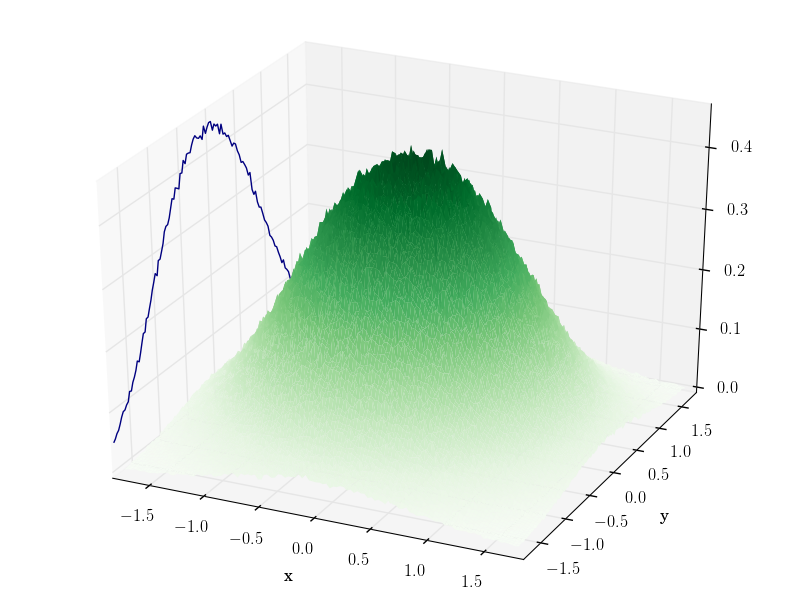
\includegraphics[scale=0.35]{../Graphics/OBD/OBD_DMC/dist_out_QDots2c1_3D.png}}
  \subfigure[$N=6$]{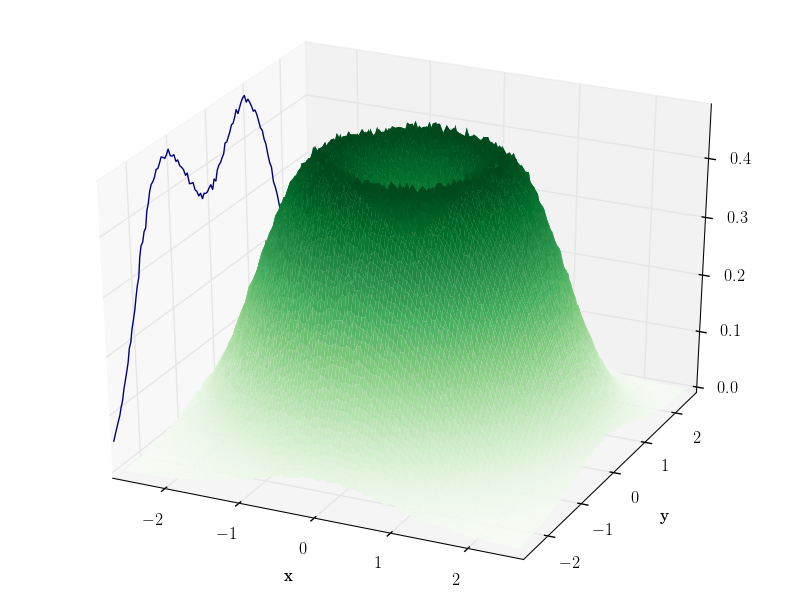
\includegraphics[scale=0.35]{../Graphics/OBD/OBD_DMC/dist_out_QDots6c1_3D.png}} \\
  \subfigure[$N=12$]{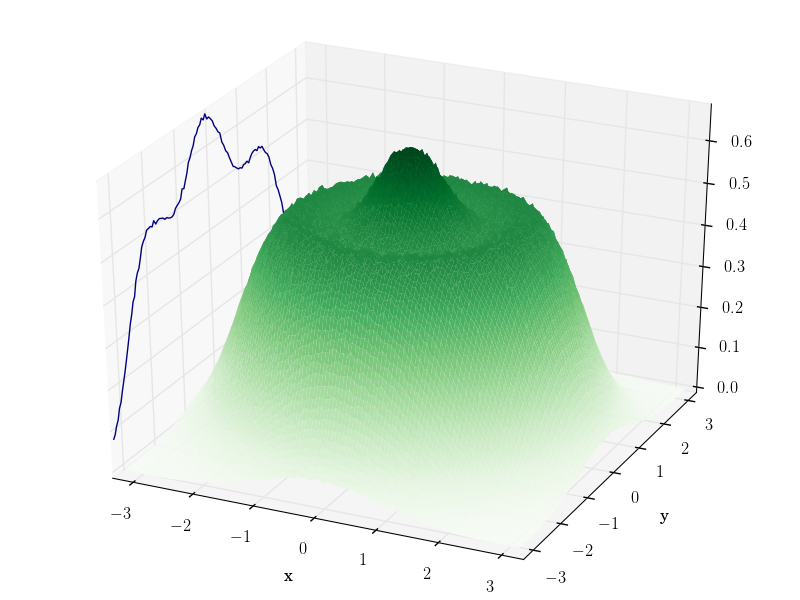
\includegraphics[scale=0.35]{../Graphics/OBD/OBD_DMC/dist_out_QDots12c1_3D.png}}
  \subfigure[$N=20$]{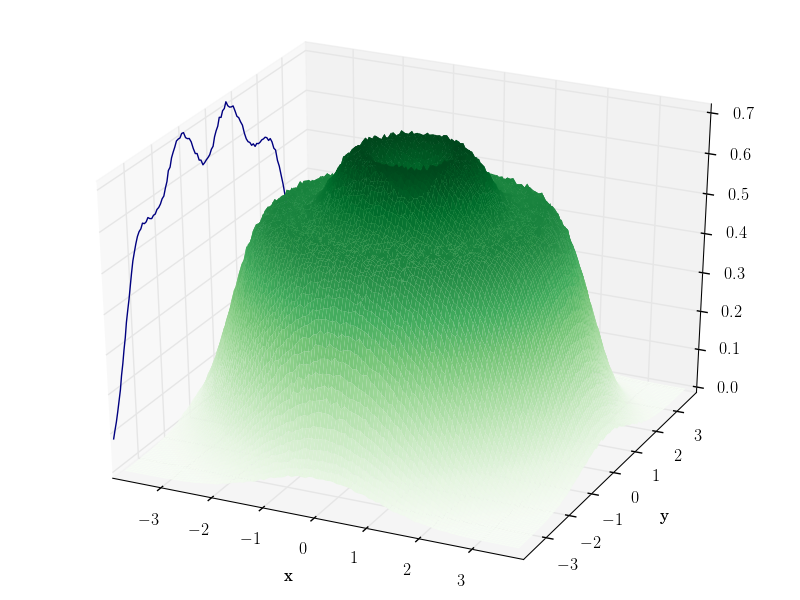
\includegraphics[scale=0.35]{../Graphics/OBD/OBD_DMC/dist_out_QDots20c1_3D.png}} \\
  \subfigure[$N=30$]{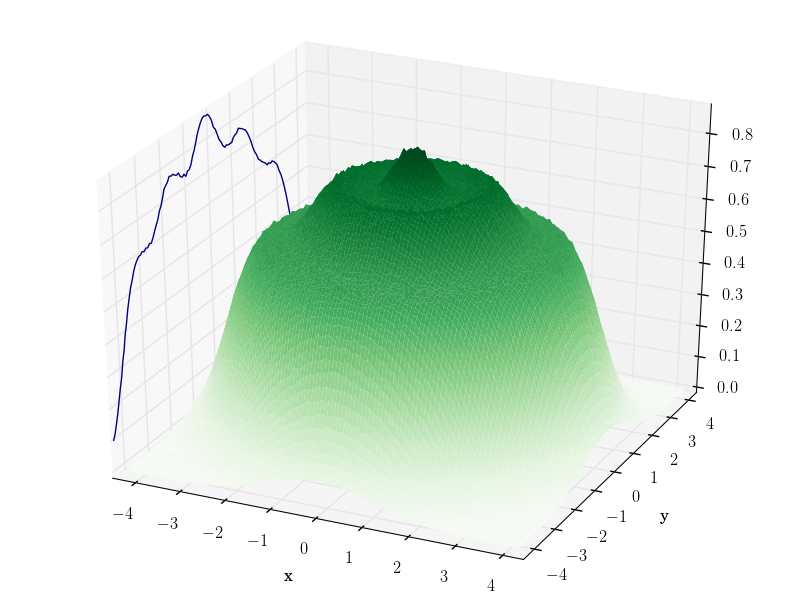
\includegraphics[scale=0.35]{../Graphics/OBD/OBD_DMC/dist_out_QDots30c1_3D.png}}
  \subfigure[$N=42$]{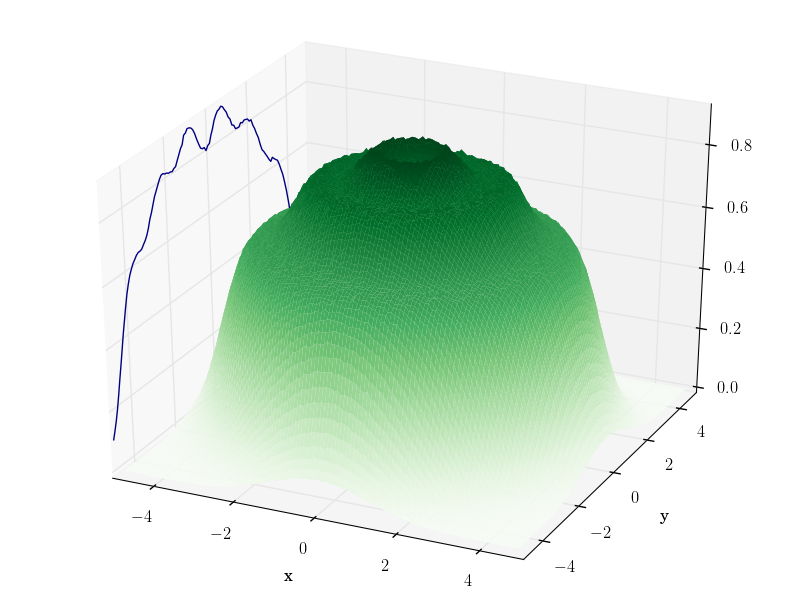
\includegraphics[scale=0.35]{../Graphics/OBD/OBD_DMC/dist_out_QDots42c1_3D.png}} \\
  \caption{Diffusion Monte-Carlo one-body densities for two-dimensional quantum dots with frequency $\omega=1$. The number of particles $N$ are listed below each density. It is apparent that the density behaves much like water ripples as the number of particles increase, conserving the shape in an oscillatory manner.}
  \label{fig:OBD_DMC_QDOTS_w1} 
 \end{center}
\end{figure}

\clearpage


Due to the electron-electron interaction, the Schrödinger equation is not separable in Cartesian coordinates. It is therefore not given that the insights from two dimensions can be transferred to the three-dimensional case. Nevertheless, by looking at the one-body densities for three dimensions in Figure \ref{fig:OBD_QDOTS3D_highfreq}, it is apparent that the general density profile is unchanged. The only thing separating two - and three-dimensional quantum dots is the number of electrons in the closed shells.

Note however, that this similarity only holds when the number of closed shells are equal. Comparing the two-dimensional density for $N=20$ electrons from Figure \ref{fig:OBD_DMC_QDOTS_w1} with the three-dimensional one for $N=20$ electrons given above, it is apparent that the shape of the densities are not conserved with respect to the number of particles $N$ alone.

% \setlength{\tabcolsep}{0.1pt}
\begin{figure}
 \begin{center}
 \begin{tabular}{cc|c}
   \subfigure{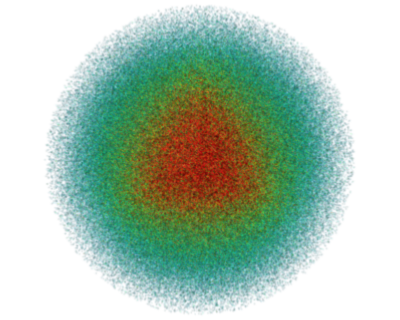
\includegraphics[scale=0.3]{../Graphics/OBD/OBD_Q3D/QD2w1_3D.png}} &
   \subfigure{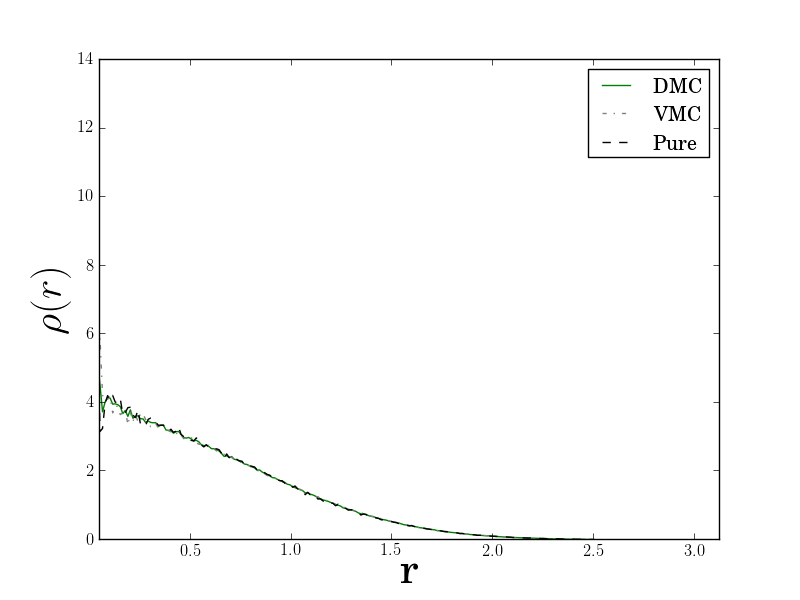
\includegraphics[scale=0.25]{../Graphics/OBD/OBD_Q3D/QD2w1_2D.png}} &
   \subfigure{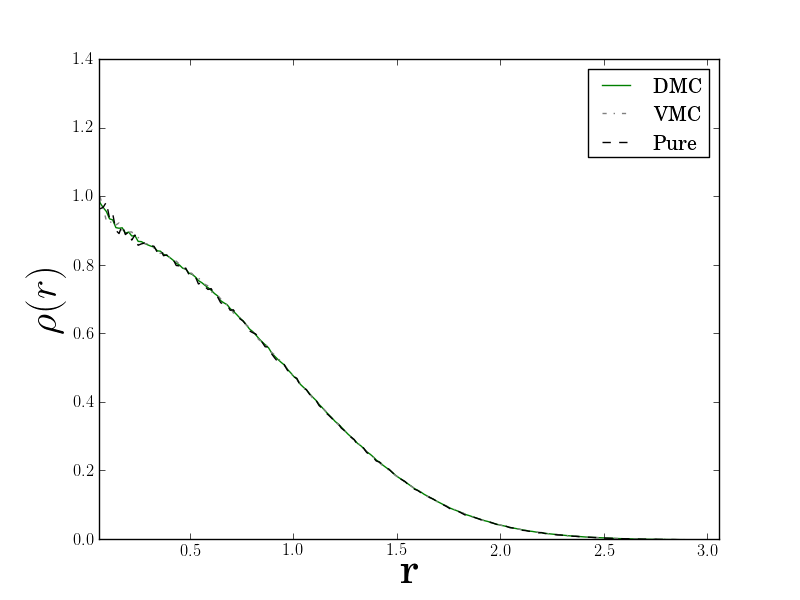
\includegraphics[scale=0.25]{../Graphics/OBD/OBD_Q3D/comp/Q2D_2.png}} \\
   \subfigure{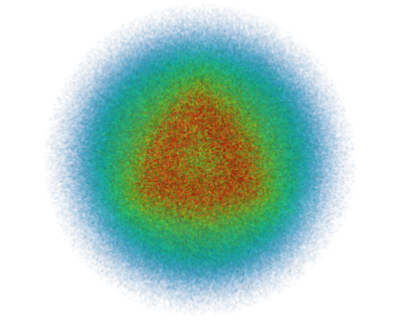
\includegraphics[scale=0.3]{../Graphics/OBD/OBD_Q3D/QD8w1_3D.png}} &
   \subfigure{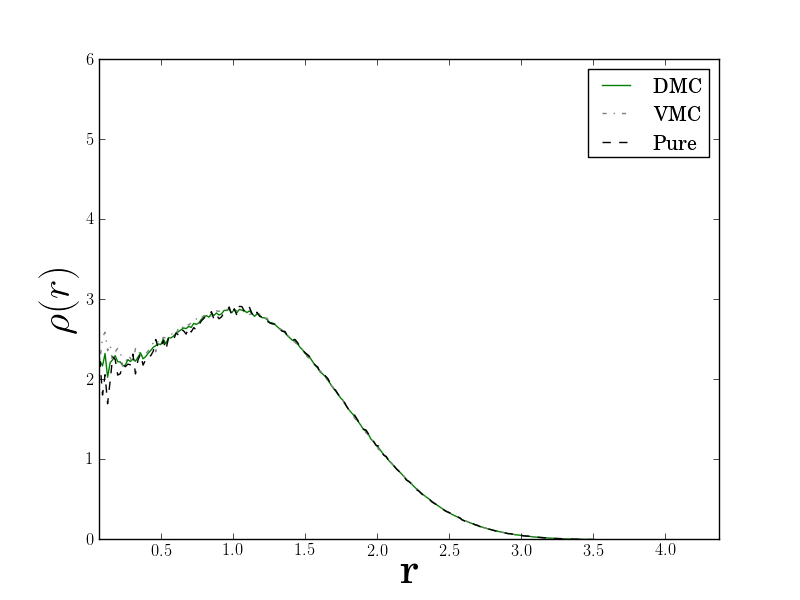
\includegraphics[scale=0.25]{../Graphics/OBD/OBD_Q3D/QD8w1_2D.png}} & 
   \subfigure{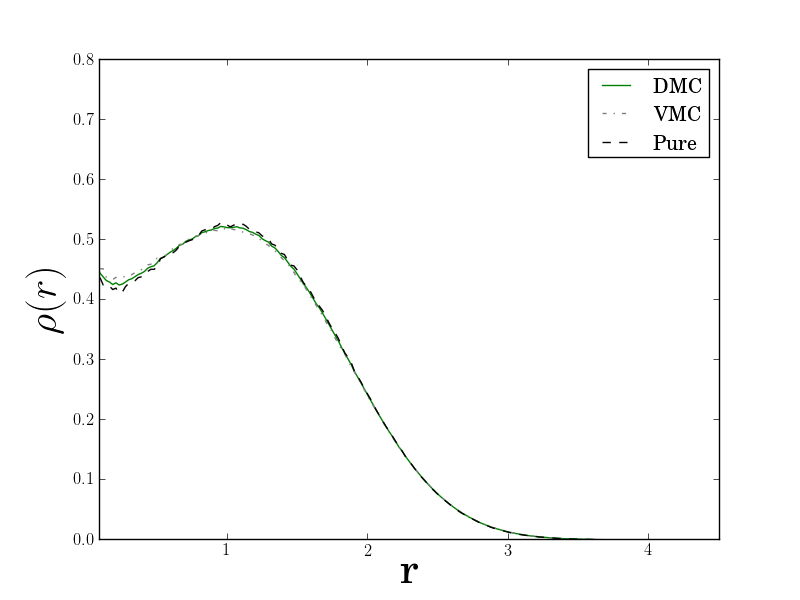
\includegraphics[scale=0.25]{../Graphics/OBD/OBD_Q3D/comp/Q2D_6.png}} \\
   \subfigure{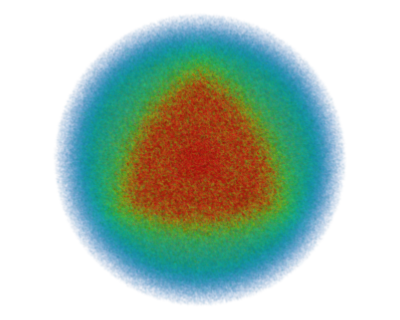
\includegraphics[scale=0.3]{../Graphics/OBD/OBD_Q3D/QD20w1_3D.png}} &
   \subfigure{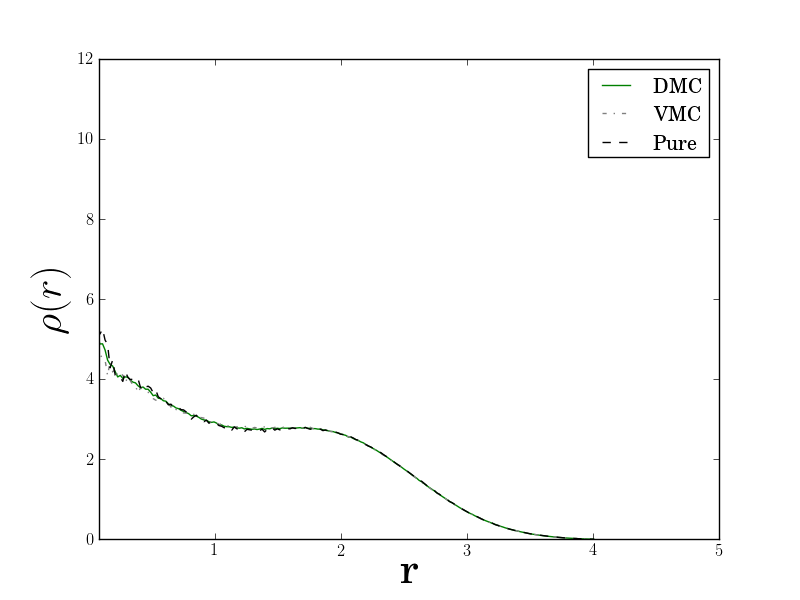
\includegraphics[scale=0.25]{../Graphics/OBD/OBD_Q3D/QD20w1_2D.png}} & 
   \subfigure{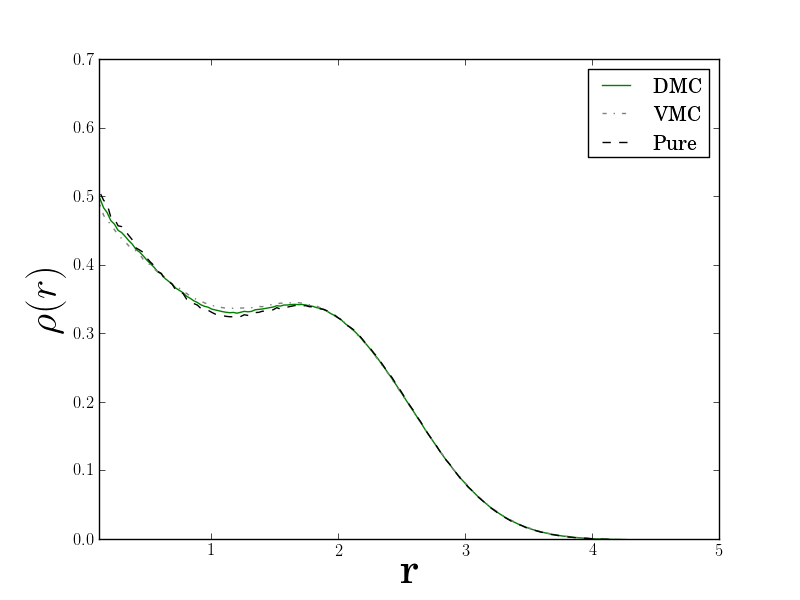
\includegraphics[scale=0.25]{../Graphics/OBD/OBD_Q3D/comp/Q2D_12.png}} \\
  \end{tabular}
  \caption{Left and middle column: One-body densities for quantum dots in three dimensions with frequency $\omega=1$. A quarter of the spherical density is removed to present a better view of the core.  Red and blue color indicate a low and high electron density, respectively. From top to bottom, the number of particles are $2$, $8$ and $20$. Right column: One-body densities for two-dimensional quantum dots for $N=2$, $6$ and $12$ electrons (from the top) with $\omega=1$. It is apparent that the  shape of the density is conserved as the third dimension is added. The radial densities are not normalized. Normalizing the densities would only change the vertical extent.}
  \label{fig:OBD_QDOTS3D_highfreq}
 \end{center}
\end{figure}
% \setlength{\tabcolsep}{pt}

\captionsetup[subfloat]{labelformat=parens}

\clearpage

\subsection{Lowering the frequency}

An interesting effect of lowering the frequency is that the two - and three-dimensional densities no longer match. For example, the radial density for the three-dimensional $N=8$ quantum dot from Figure \ref{fig:OBD_QDOTS3D_highfreq} was a near perfect match to the two-dimensional one for $N=6$ electrons, however, comparing the same densities for $\omega=0.01$ from Figures \ref{fig:OBD_QDOTS3D_lowfreq} and \ref{fig:OBD_DMC_QDOTS_lowering3D}, it is apparent that this is no longer the case; the two-dimensional density has a peak in the center region, whereas the three-dimensional density is zero in the center region.

From Figure \ref{fig:OBD_QDOTS3D_lowfreq} it is apparent that lowering the frequency increases the radial extent of the quantum dot, and thus lowers the electron density. Moreover, Figure \ref{fig:OBD_DMC_QDOTS_lowering3D} reveals that the electron density becomes similar in height and more localized across the quantum dot, which implies that the electrons on average are spread evenly in shell structures. The localization of the electrons is further verified in Figure \ref{fig:E_dist_qdots}, where is is clear that the expectation value of the total potential energy becomes larger than the corresponding kinetic energy.

In order words, an evenly spread and localized electron density gives rise to \textit{crystallization}\footnote{Unless at least one particle is frozen in the QMC simulations, the quantum dot densities should always be rotationally symmetric. Crystallization in a QMC perspective comes thus not in the form of actual ``crystals'', but rather as a rotated crystallized state.}. The idea of an electron crystal was originally proposed by Wigner \cite{WignerCrystalOrig}, hence the currently discussed phenomenon is referred to as a \textit{Wigner molecule} or a \textit{Wigner crystal}, which is expected for quantum dots in the limit of low electron densities where the total potential energy dominates over the kinetic energy \cite{WignerTransport, WignerPathTo, WignerSymmetryBreak, WignerFloating, Wigner2DQD}. These electronic crystals have been observed in experiments with for example liquid helium \cite{WignerExptHelium} and semiconductors \cite{WignerExptSemicond}.

\newcommand{\qqq}{\qquad\qquad\qquad}
\newcommand{\qq}{\qquad\qquad}
\newcommand{\rot}[1]{\begin{sideways}#1\end{sideways}}
\setlength{\tabcolsep}{0.1pt}
\begin{figure}
 \begin{center}
 \begin{tabular}{rl}
   \rot{$\qq\quad\omega=1$}&\subfigure{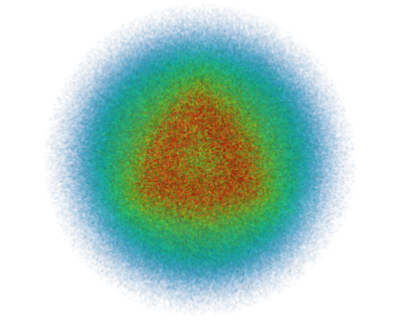
\includegraphics[scale=0.35]{../Graphics/OBD/OBD_Q3D/QD8w1_3D.png}}
   \subfigure{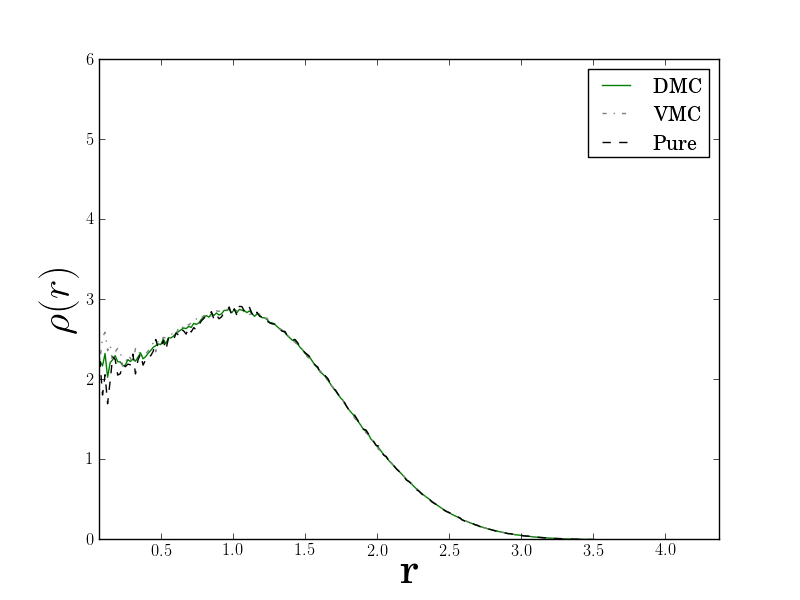
\includegraphics[scale=0.28]{../Graphics/OBD/OBD_Q3D/QD8w1_2D.png}} \\
   \rot{$\qq\omega=0.01$} &\subfigure{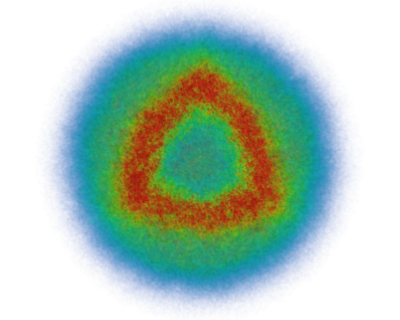
\includegraphics[scale=0.35]{../Graphics/OBD/OBD_Q3D/QD8w001_3D.png}} 
   \subfigure{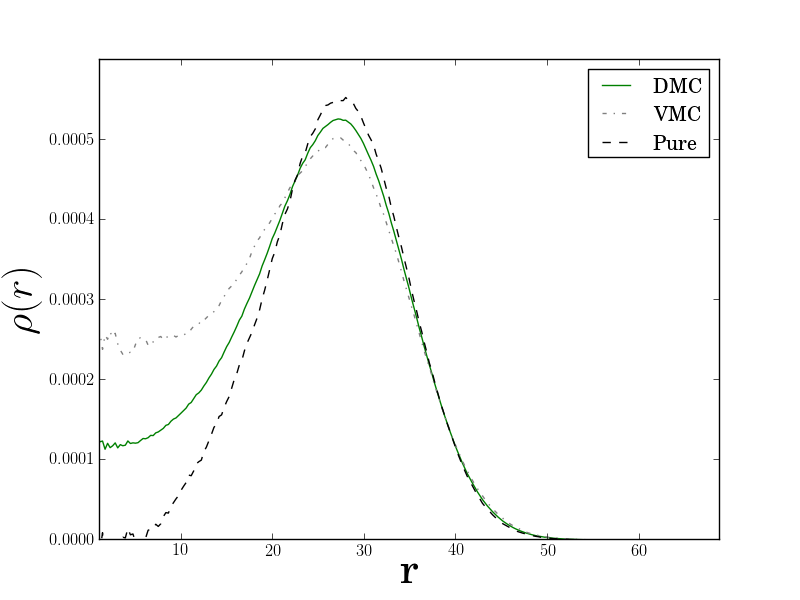
\includegraphics[scale=0.28]{../Graphics/OBD/OBD_Q3D/QD8w001_2D.png}}  \\
  \end{tabular}
  \caption{Comparison of the one-body densities for quantum dots in three dimensions for $N=8$ electrons for high and low frequency $\omega$. It is apparent that the distribution becomes more narrow as the frequency is reduced. Red and blue color indicate a low and high electron density, respectively. A quarter of the spherical density is removed to present a better view of the core. }
  \label{fig:OBD_QDOTS3D_lowfreq}
 \end{center}
\end{figure}

\captionsetup[subfloat]{labelformat=empty}
\newcommand{\OBDscale}{0.25}
\begin{landscape}
 \begin{figure}
 \begin{center}
 \begin{tabular}{rl}
  \rot{$\qquad\quad\omega=0.28$}&\subfigure{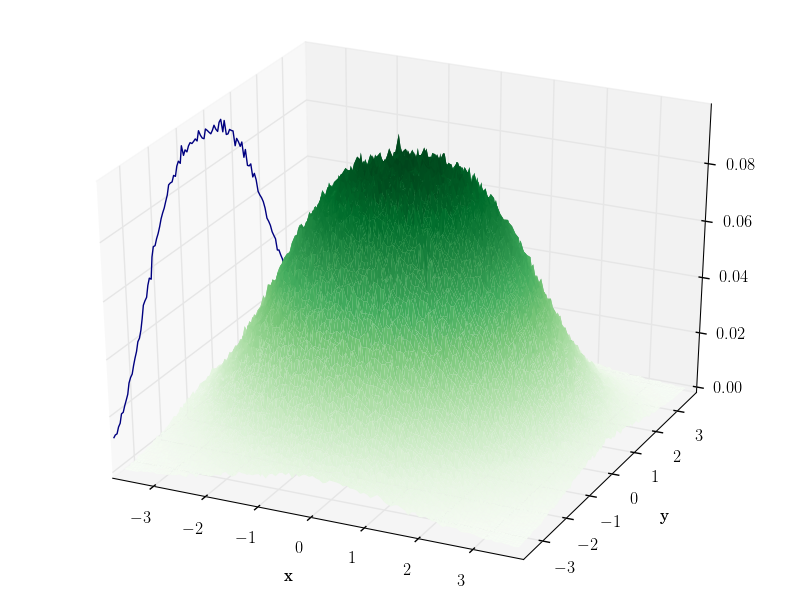
\includegraphics[scale=\OBDscale]{../Graphics/OBD/OBD_DMC/dist_out_QDots2c028_3D.png}}
  \subfigure{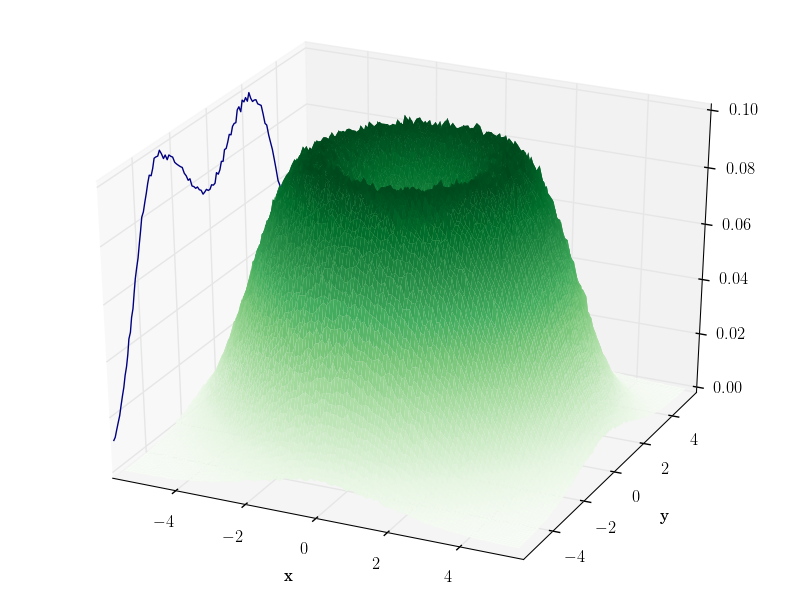
\includegraphics[scale=\OBDscale]{../Graphics/OBD/OBD_DMC/dist_out_QDots6c028_3D.png}} 
  \subfigure{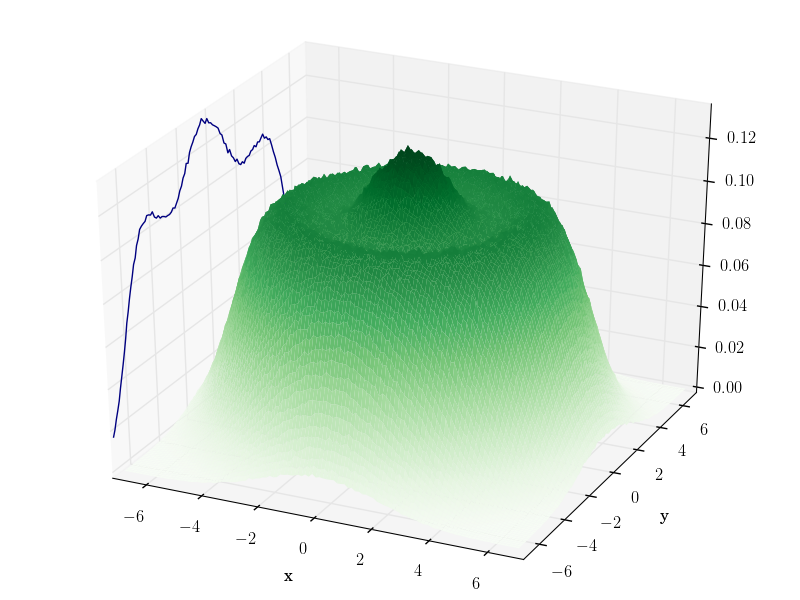
\includegraphics[scale=\OBDscale]{../Graphics/OBD/OBD_DMC/dist_out_QDots12c028_3D.png}}
  \subfigure{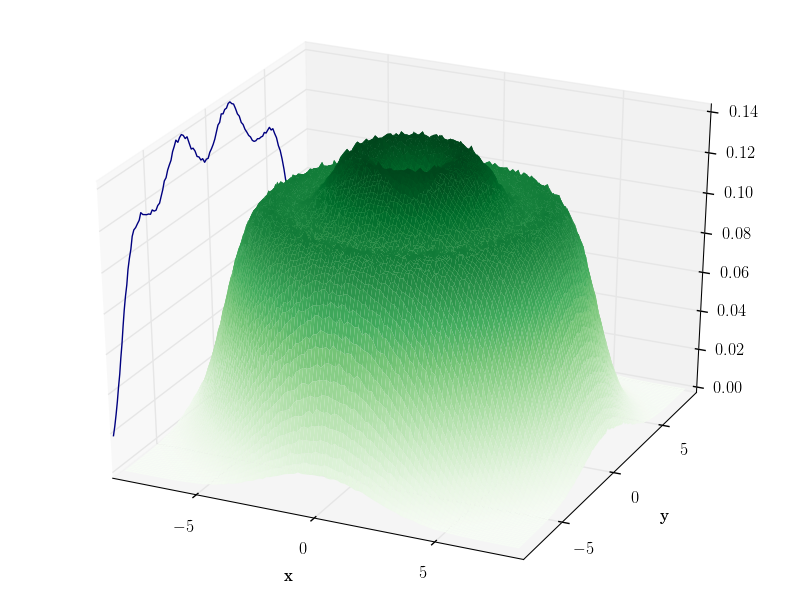
\includegraphics[scale=\OBDscale]{../Graphics/OBD/OBD_DMC/dist_out_QDots20c028_3D.png}} \\[-0pt]
  \rot{$\qquad\quad\omega=0.1$}&\subfigure{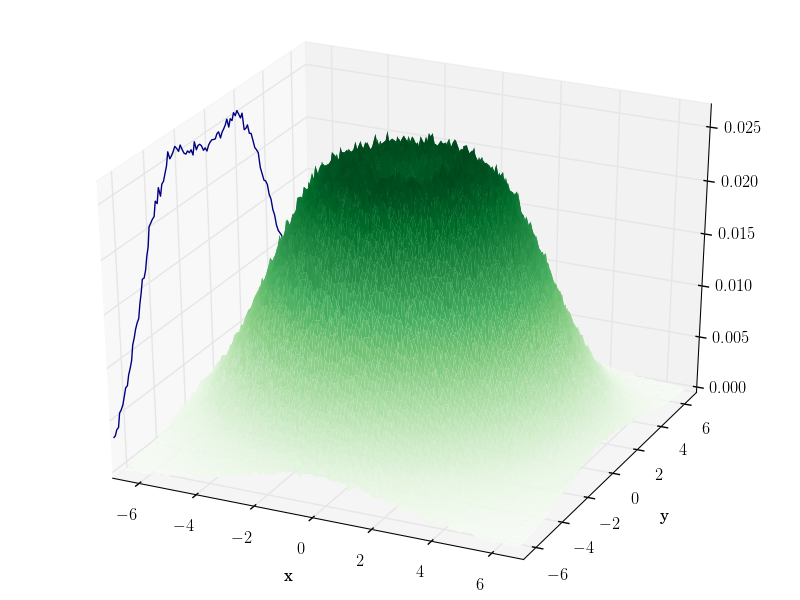
\includegraphics[scale=\OBDscale]{../Graphics/OBD/OBD_DMC/dist_out_QDots2c01_3D.png}}
  \subfigure{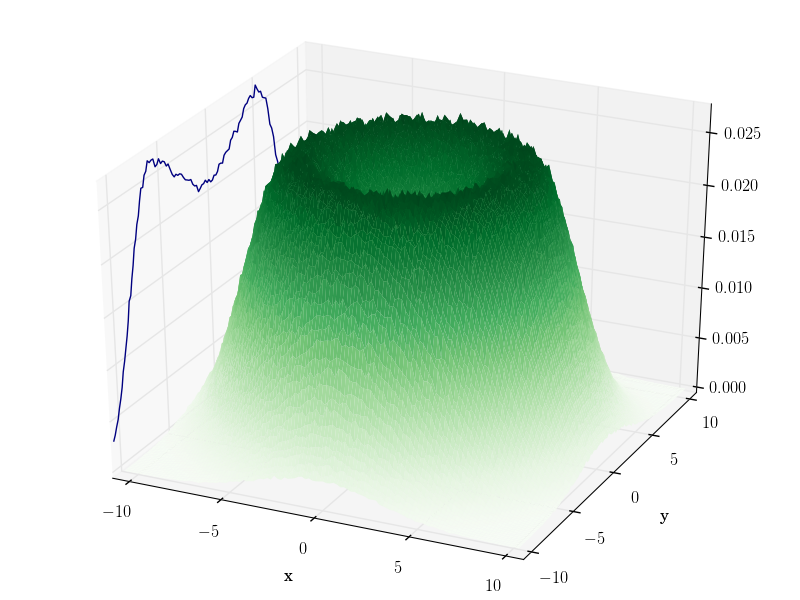
\includegraphics[scale=\OBDscale]{../Graphics/OBD/OBD_DMC/dist_out_QDots6c01_3D.png}} 
  \subfigure{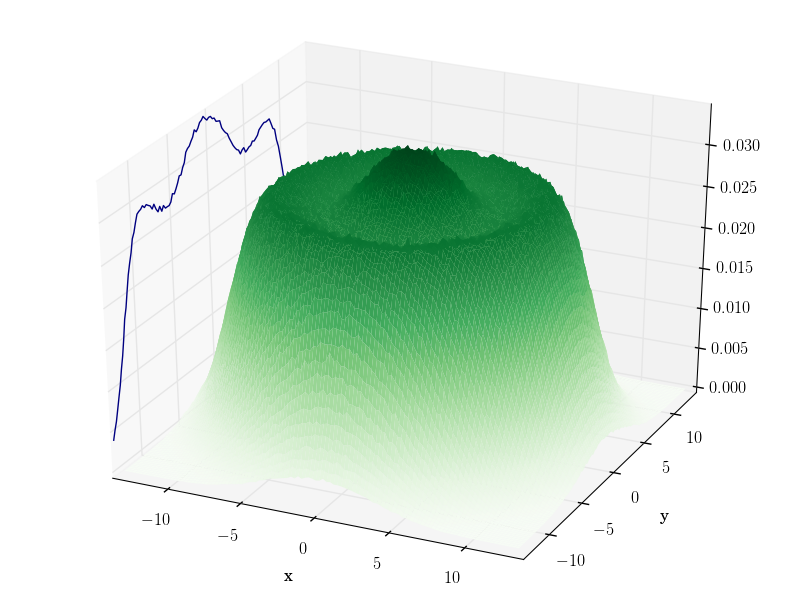
\includegraphics[scale=\OBDscale]{../Graphics/OBD/OBD_DMC/dist_out_QDots12c01_3D.png}}
  \subfigure{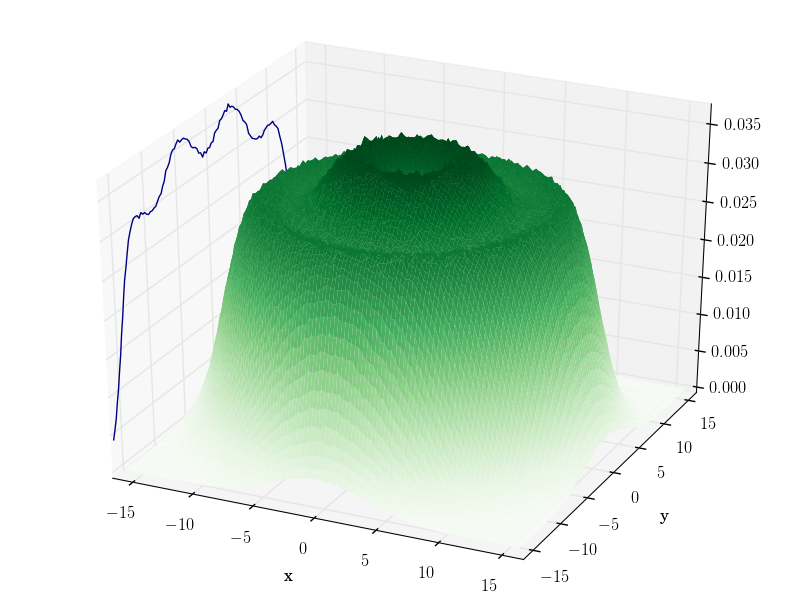
\includegraphics[scale=\OBDscale]{../Graphics/OBD/OBD_DMC/dist_out_QDots20c01_3D.png}} \\[-0pt]
  \rot{$\qquad\quad\omega=0.01$}&\subfigure[$N=2$]{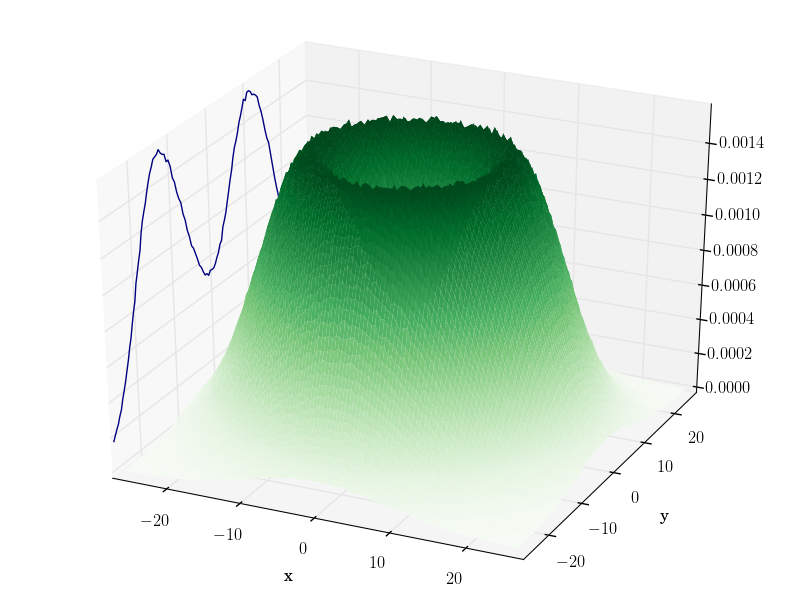
\includegraphics[scale=\OBDscale]{../Graphics/OBD/OBD_DMC/dist_out_QDots2c001_3D.png}}
  \subfigure[$N=6$]{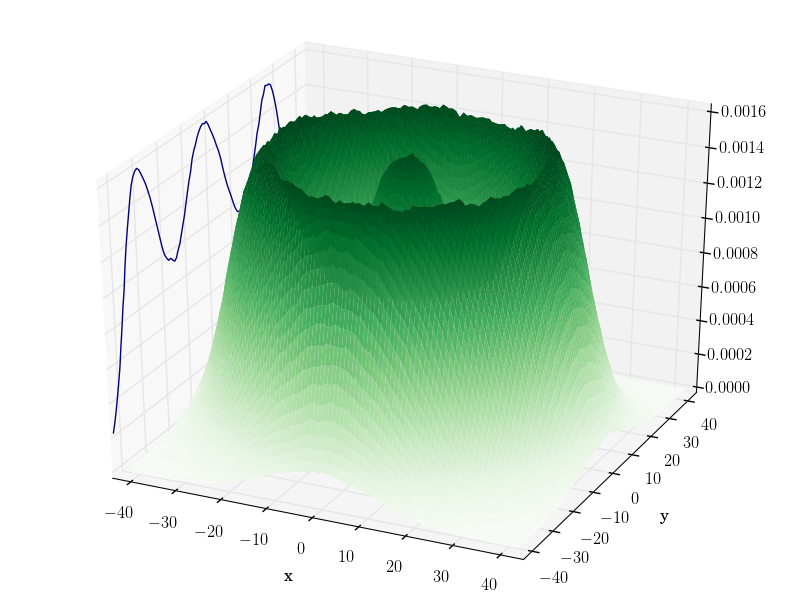
\includegraphics[scale=\OBDscale]{../Graphics/OBD/OBD_DMC/dist_out_QDots6c001_3D.png}} 
  \subfigure[$N=12$]{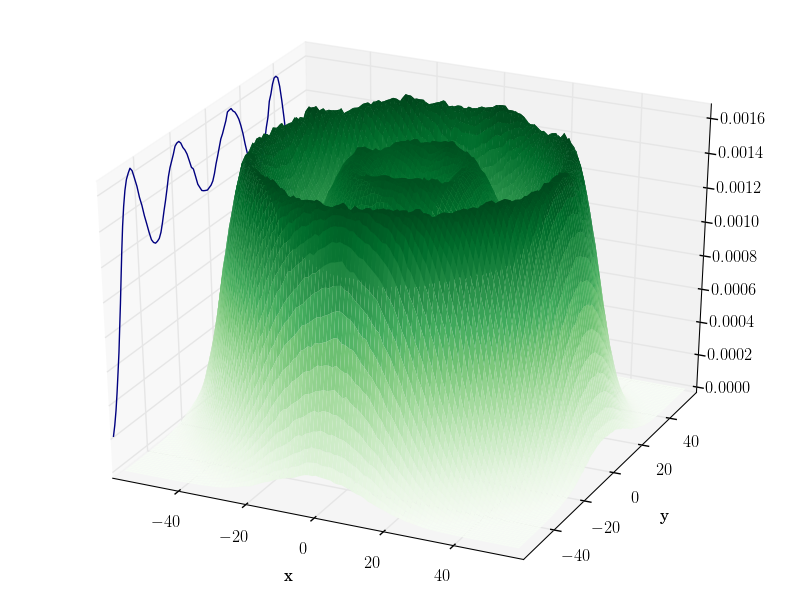
\includegraphics[scale=\OBDscale]{../Graphics/OBD/OBD_DMC/dist_out_QDots12c001_3D.png}}
  \subfigure[$N=20$]{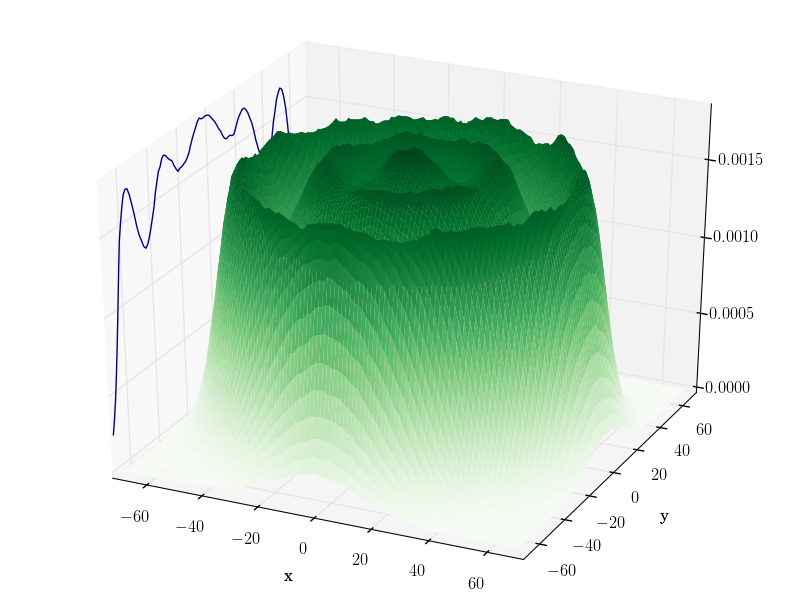
\includegraphics[scale=\OBDscale]{../Graphics/OBD/OBD_DMC/dist_out_QDots20c001_3D.png}} \\
 \end{tabular}
  \caption{\small{DMC One-body densities for Quantum Dots for decreasing oscillator frequencies $\omega$ and increasing number of particles $N$. Each row represents a given $\omega$, and each column represents a given $N$. Notice that the densities for $\omega=1$ (from Figure \ref{fig:OBD_DMC_QDOTS_w1}) are indistinguishable from those of $\omega=0.28$ except for their radial extent. This trend has been verified in the case of $N=30$, 42 and 56 electrons as well as for $\omega=0.5$, however, for the sake of transparency, these results are left out of the current figure.}}
  \label{fig:OBD_DMC_QDOTS_lowering3D}
 \end{center}
\end{figure}
\end{landscape}

\captionsetup[subfloat]{labelformat=parens}
\setlength{\tabcolsep}{6pt}


\captionsetup[subfloat]{labelformat=empty}
\begin{figure}[h]
 \begin{center}
  \subfigure[$N=6$]{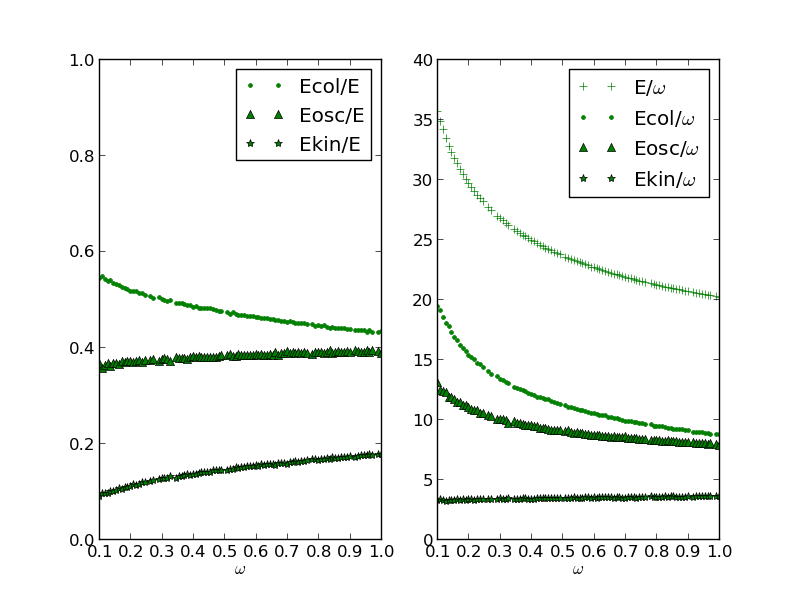
\includegraphics[scale=0.35]{../Graphics/VirialPlots/E_vs_w_E6.png}}
  \subfigure[$N=42$]{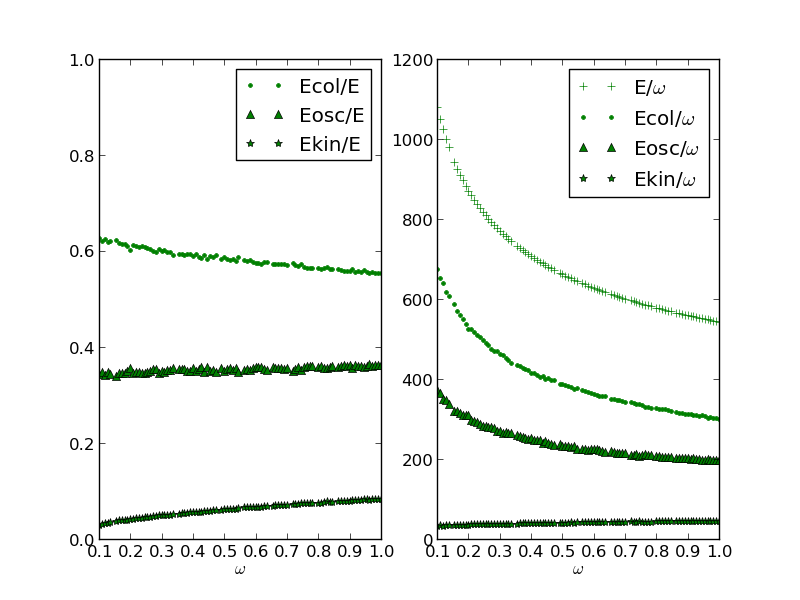
\includegraphics[scale=0.35]{../Graphics/VirialPlots/E_vs_w_E42.png}} \\
  \caption{The relative magnitude of the expectation value of the different energy sources as a function of the frequency $\omega$ (left) together with the magnitude of the sources' energy contributions scaled with the oscillator frequency (right). The plots are supplied with legends to increase the readability. The different energy sources are the kinetic energy denoted \textit{Ekin}, the oscillator potential energy denonted \textit{Eosc}, and the electron-electron interaction energy denoted \textit{Ecol}. Note that all given energies are expectation values. The values are calculated using two-dimensional quantum dots. The number of electrons $N$ is displayed beneath each respective plot. It is apparent that the kinetic energy contribution is constant in both cases. Moreover, the oscillator potential contribution is more or less constant for the relative energies (left sub-figures). The figure clearly indicates that the potential energy contributions from the oscillator and the electron-electron interaction 
tends to dominate over the kinetic energy at lower frequencies.}
  \label{fig:E_dist_qdots}
 \end{center}
\end{figure}

It is expected that the QMC Wigner crystal corresponds to the electrons localizing around the equilibrium positions of the classical Wigner crystal\cite{WignerTransport}. Comparing the densities for two-dimensional quantum dots at $\omega=0.01$ for $N=6$, $12$, and $20$ electrons given in Figure \ref{fig:OBD_DMC_QDOTS_lowering3D} to similar classical calculations done in Ref. \cite{WignerClassic} for $N=6$, $10$, and $19$ electrons, respectively, it is apparent that the solutions match very well.  

It was mentioned previously that the Wigner crystallization of quantum dots came as a consequence of the average total potential energy being larger than the corresponding kinetic energy. This relationship between kinetic - and potential energy is closely related to the \textit{virial theorem} from classical mechanics. The quantum mechanical version of the virial theorem was proven by Fock in 1930 \cite{FockVirial} and reads

\begin{equation}
 V(\mathbf{r}) \propto r^\gamma \quad\longrightarrow\quad \langle \OP{T} \rangle = \frac{\gamma}{2} \langle \OP{V} \rangle, \label{eq:virial}
\end{equation}

where $\OP{T}$ and $\OP{V}$ denote the kinetic - and total potential energy operators, respectively. The important conclusion which can be drawn from this is that if two systems have an equal ratio of kinetic - to total potential energy, the systems behave identically in the sense that they follow the same effective potential, and thus have similar eigenstates. 

From Figure \ref{fig:V_dist_qdots} it is apparent that there is a remarkably constant slope for two different regions in the case of quantum dots, namely high - and low kinetic energy, which by looking at Figure \ref{fig:E_dist_qdots} corresponds to high - and low frequencies. In light of previous discussions, one may suggest that the change in the slopes
of Figure \ref{fig:V_dist_qdots} corresponds to the quantum dot system  making a transition into a Wigner crystallized state.



\newpage

\begin{figure}[h]
 \begin{center}
  \subfigure[$N=6$]{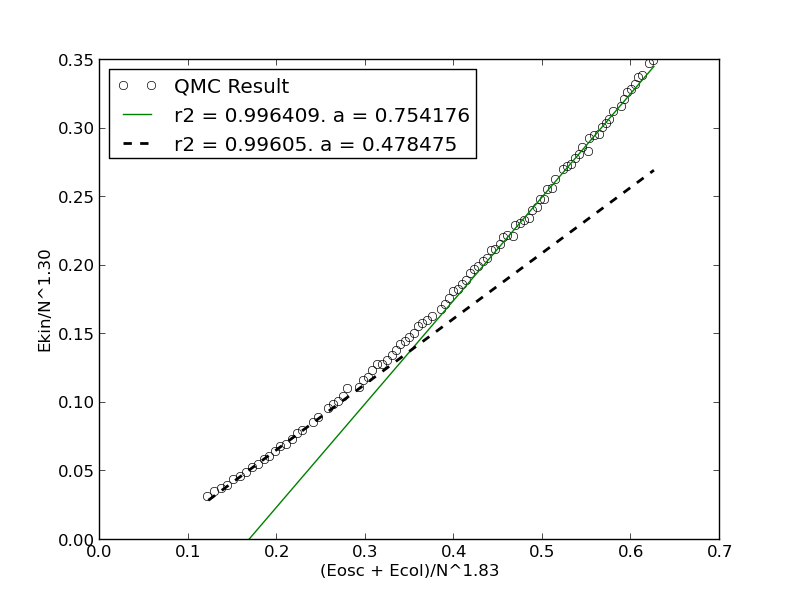
\includegraphics[scale=0.35]{../Graphics/VirialPlots/E_vs_w_V6.png}}
  \subfigure[$N=42$]{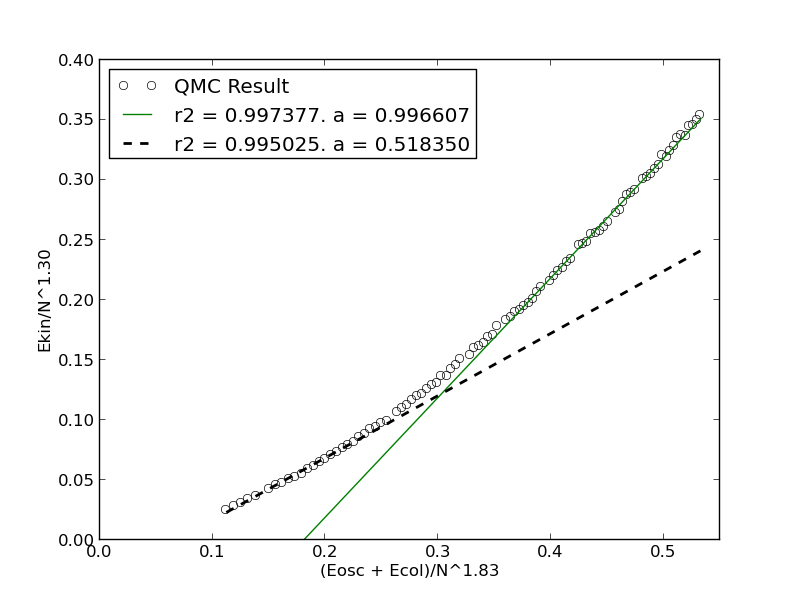
\includegraphics[scale=0.35]{../Graphics/VirialPlots/E_vs_w_V42.png}} \\
  \caption{The total kinetic energy vs. the total potential energy of two-dimensional quantum dots. The number of electrons $N$ are displayed beneath each respective plot. The axes are scaled with a power of $N$ to collapse the data to the same axis span. Once the kinetic energy drops below a certain energy dependent on the number of particles, the slope changes, which in light of the virial theorem from Eq.~(\ref{eq:virial}) indicates that the overall system changes properties. The data is fitted to linear lines with resulting slopes $a$ displayed in the legend. The parameter $r2$ indicates how well the data fits a linear line. An exact fit yields $r2 = 1$.}
  \label{fig:V_dist_qdots}
 \end{center}
\end{figure}
\captionsetup[subfloat]{labelformat=parens}

\subsection{Simulating a Double-well}

\begin{figure}[h]
 \begin{center}
 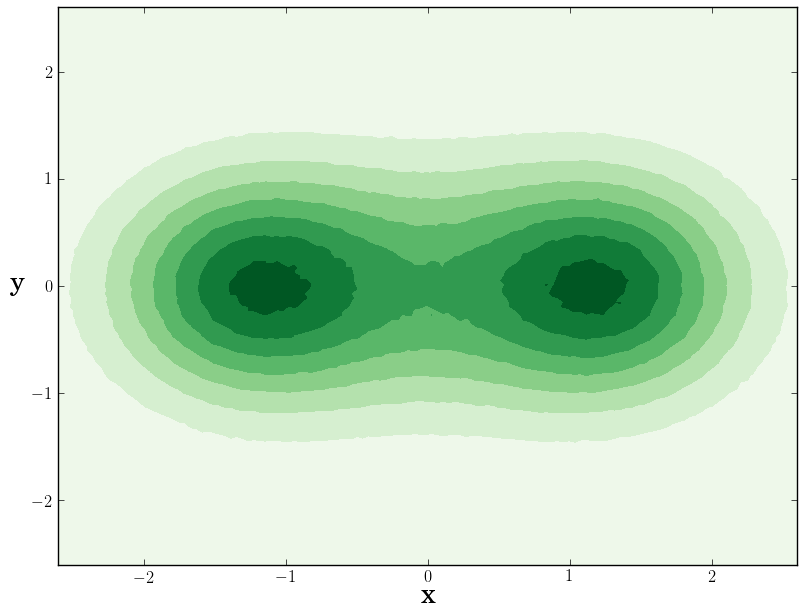
\includegraphics[scale=0.35]{../Graphics/DoubleWell.png}
  \caption{A countour plot of the trial wave function for a two-particle double-well quantum dot with the wells separated at a distance $R = 2$ in the $x$-direction using $m^\ast = \omega_0 = 1$. See Section \ref{sec:modelQDots} for an introduction to the double well potential. It is apparent that there is one electron located in each well, however, with a slight overlap in the middle region.}
  \label{fig:doubleWell}
 \end{center}
\end{figure}
\captionsetup[subfloat]{labelformat=parens}

Figure \ref{fig:doubleWell} shows the distribution for a two-particle simulation. It is apparent that despite the wells being separated, their local distributions overlap, indicating that the electrons can \textit{tunnel}, that is, they have a non-zero probability of appearing on the other side of the barrier. Comparing the distribution to the potential in Figure \ref{fig:extPotDoubleWell}, it is clear that they match very well.

The DMC result is $\mathrm{E_{DMC}} = 2.3496(1)$, whereas the non-interacting energy is $E_0 = 2$ and the single-well energy is $E_0=3.0$. It is expected that the energy lands in between these, as $R=0$ corresponds to the single well and $R\to\infty$ corresponds to the non-interacting case. 

\clearpage
\section{Atoms}
 
 The focus regarding atoms has been on simulating heavy atoms using a simple ansatz for the trial wave function, and thus test its limits. Due to the importance of atoms in nature, precise calculations which are believed to be very close to the exact result for the given Hamiltonian are done. These results will be featured as experimental results in the following discussions. For heavier atoms, relativistic effects become important due to the high energies of the valance electrons. Hence atoms heavier than krypton have not been studied. The specifics regarding the model used for atoms are given in Section \ref{sec:modelAtoms}.
 
\subsection{Ground State Energies}
 
 Table \ref{tab:AtomsRes} presents the ground state energy results for different atoms together with the experimental results. As expected, helium has the best match with the corresponding experimental result out of all the atoms. The relative precision of the heavier atoms are in the range $10^{-3}$ - $10^{-4}$, indicating that DMC performs equally well in all cases. However, the error in the calculations increases as the atoms become heavier. The calculations were done on a single node; running the calculations on several nodes with an increased number of walkers could reduce the errors somewhat. 
 
 In comparison to quantum dots, where the VMC and DMC results were relatively similar, it is evident that VMC performs rather poorly compared to DMC for atoms. Unlike quantum dots, the atomic systems allow for unbound states. This implies that the atomic systems in this thesis have an additional approximation in the trial wave function due to the fact that all the orbitals represent bound states. Nevertheless, this only further demonstrate the strengths of DMC to predict accurate results without much knowledge of the system at hand.
 
\begin{table}
\begin{center}
\begin{tabular}{lp{2cm}cclc}
Atom & & $E_\mathrm{VMC}$ & \qquad $E_\mathrm{DMC}$ & \qquad\,\, Expt. & \qquad $\epsilon_\mathrm{rel}$\\
\hline\hline
\ \\
He & \qquad & -2.8903(2) & \qquad -2.9036(2) & \qquad $-2.9037$ & \qquad $3.44\cdot 10^{-5}$\\
\ \\
Be & \qquad & -14.145(2) & \qquad -14.657(2)  & \qquad $-14.6674$ & \qquad $7.10\cdot 10^{-4}$ \\
\ \\
Ne & \qquad & -127.853(2) & \qquad -128.765(4) & \qquad $-128.9383$ & \qquad $1.34\cdot 10^{-3}$  \\
\ \\
Mg & \qquad & -197.269(3) & \qquad -199.904(8) & \qquad $-200.054$ & \qquad $7.50\cdot 10^{-4}$  \\
\ \\
Ar & \qquad & -524.16(7) & \qquad -527.30(4) & \qquad $-527.544$ & \qquad $4.63\cdot 10^{-4}$  \\
\ \\
Kr & \qquad & -2700(5) & \qquad -2749.9(2) & \qquad $-2752.054976$ & \qquad $7.83\cdot 10^{-4}$  \\
\ \\
\end{tabular}
\caption{Ground state energies for Atoms calculated using Variational - and Diffusion Monte-Carlo. Experimental energies are listed in the last column. As we see, DMC is rather close to the experimental energy. The relative error $\epsilon_\mathrm{rel} = |E_\mathrm{DMC} - \mathrm{Expt.}|/|\mathrm{Expt.}|$ is as expected lowest in the case of helium. The experimental energies, that is, the best possible results available, are taken from Ref. \cite{AtomsExact} for He through Ar, and \cite{KryptonExact} for Kr. }
\label{tab:AtomsRes}
\end{center}
\end{table}
 
 
 \subsection{One-body densities}
 
 The one-body densities for the \textit{noble gases}, that is, the closed shell atoms, are presented in Figure \ref{fig:OBD_noble_Atoms_2D_combo}. Comparing these to the one-body densities for the alkaline earth metals, i.e.~$\mathrm{Be}$, $\mathrm{Mg}$, etc., in Figure \ref{fig:OBD_alkaline_Atoms_2D_combo}, it is clear that the noble gases have a more confined electron distribution. This corresponds well to the fact that noble gases do not form compound materials, i.e.~molecules \cite{UniversityPhysics}. The alkaline earth metals, on the other hand, are found naturally as parts of compound materials. The one-body densities of the alkaline earth metals spreading out in space are thus in excellent agreement with what is expected.
 
It is apparent that the VMC distribution and the pure distribution differ more in the case of alkaline earth metals than for noble gases. This implies that the trial wave function is better in the case of noble gases. To explain this phenomenon, it is important to realize that for closed shell systems, which is the case of noble gases, the energy needed to excite an electron into the next $n$-shell is higher than the energy needed to excite an electron to the next $l$-level in an open shell system such as the alkaline earth metals. The result of this is that the contributions from the exited states to the total wave function in Eq.~(\ref{eq:MultiDeterminantTWF}) are higher for the alkaline earth metals than for the noble gases. This is exactly the same scenario as for high and low frequency quantum dots.

The approximation made in this thesis is that the trial wave function consists of a single determinant, thus neglecting the contribution from excited states. In light of the above discussion, this approximation is in other words better for noble gases than for the alkaline earth metals.
 
 
 
 \begin{figure}
 \begin{center}
   \subfigure{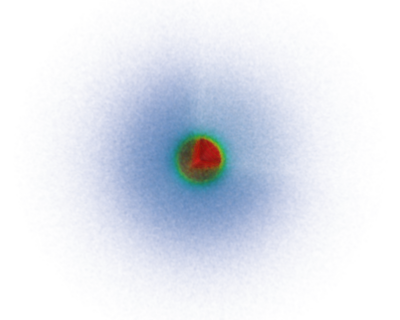
\includegraphics[scale=0.4]{../Graphics/OBD/OBD_Atoms/3D/Beryllium.png}} 
   \subfigure{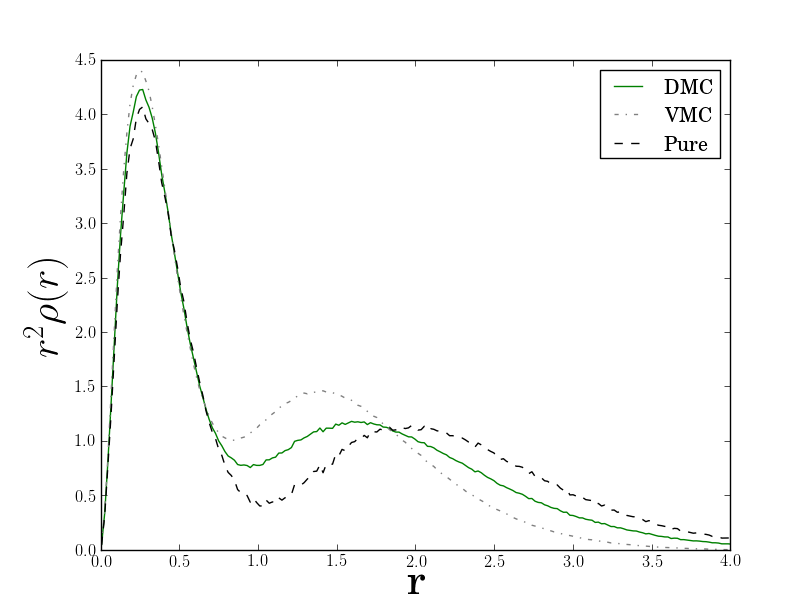
\includegraphics[scale=0.3]{../Graphics/OBD/OBD_Atoms/2D/Beryllium.png}}  \\
   \subfigure{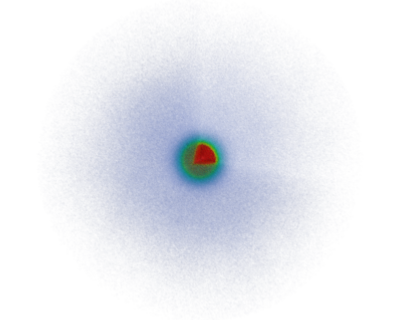
\includegraphics[scale=0.4]{../Graphics/OBD/OBD_Atoms/3D/Magnesium.png}} 
   \subfigure{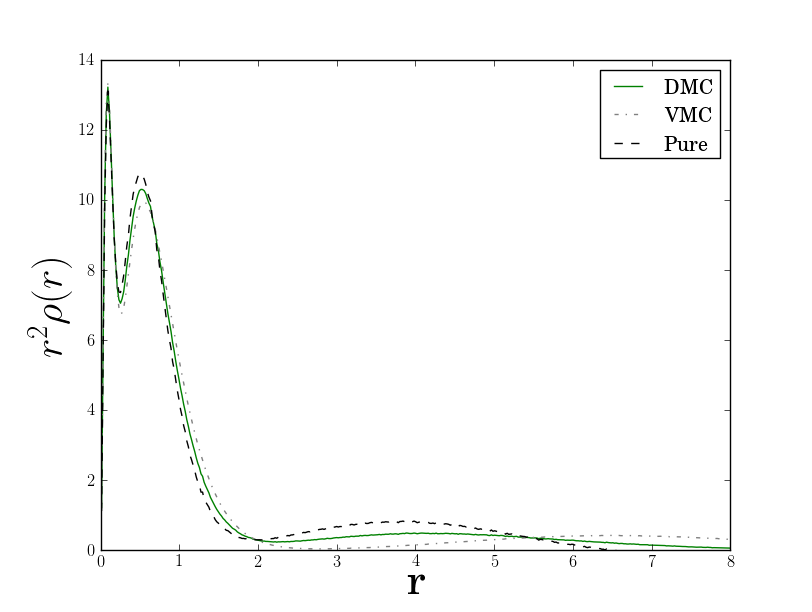
\includegraphics[scale=0.3]{../Graphics/OBD/OBD_Atoms/2D/Magnesium.png}}  \\
  \caption{Three dimensional one-body densities (left column) and radial densities (right column) for alkaline earth metals; beryllium (top) and magnesium (bottom). A quarter of the spherical density is removed to present a better view of the core. Notice that the radial one-body densities in the right column are multiplied by the radius squared. This is done in order to reveal the characteristics behind a density which otherwise is a generic peak around the origin. Compared to the noble gases in Figure \ref{fig:OBD_noble_Atoms_2D_combo}, the alkaline earth metals have a surrounding dispersed probability cloud due to having easily excitable valence electrons. The element is thus more unstable and potent for chemical reactions and molecular formations through covalent - and ionic bonds \cite{UniversityPhysics}. Red and blue color indicate a low and high electron density, respectively.}
  \label{fig:OBD_alkaline_Atoms_2D_combo}
 \end{center}
\end{figure}
 
\begin{figure}
 \begin{center}
   \subfigure{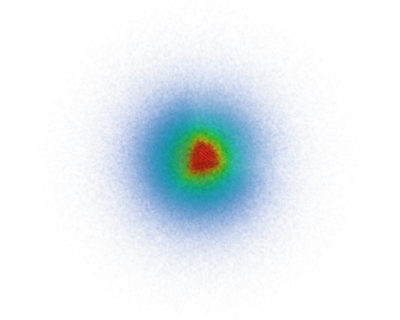
\includegraphics[scale=0.4]{../Graphics/OBD/OBD_Atoms/3D/Helium.png}} 
   \subfigure{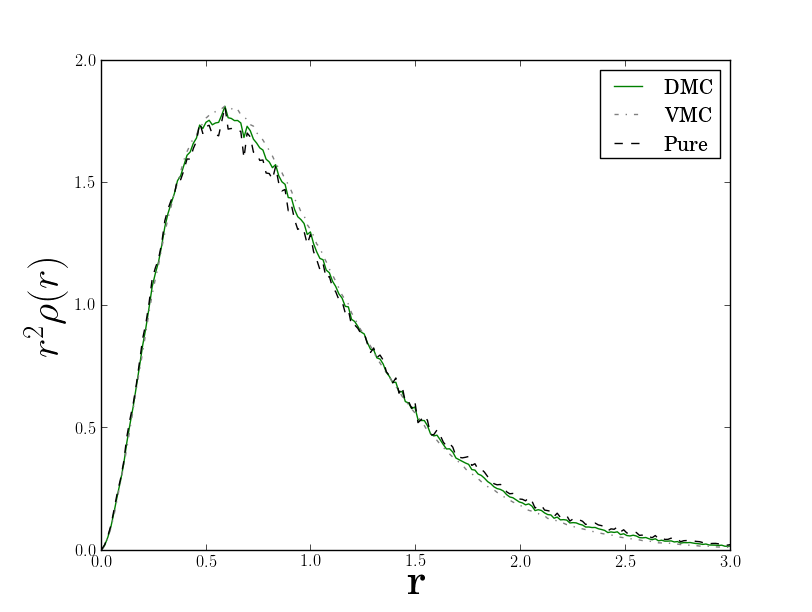
\includegraphics[scale=0.3]{../Graphics/OBD/OBD_Atoms/2D/Helium.png}}  \\
   \subfigure{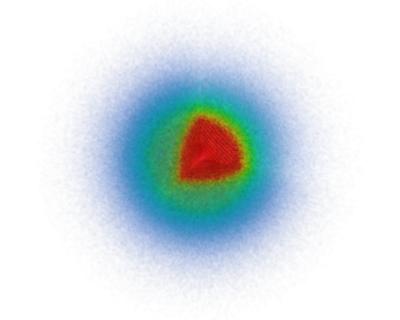
\includegraphics[scale=0.4]{../Graphics/OBD/OBD_Atoms/3D/Neon.png}} 
   \subfigure{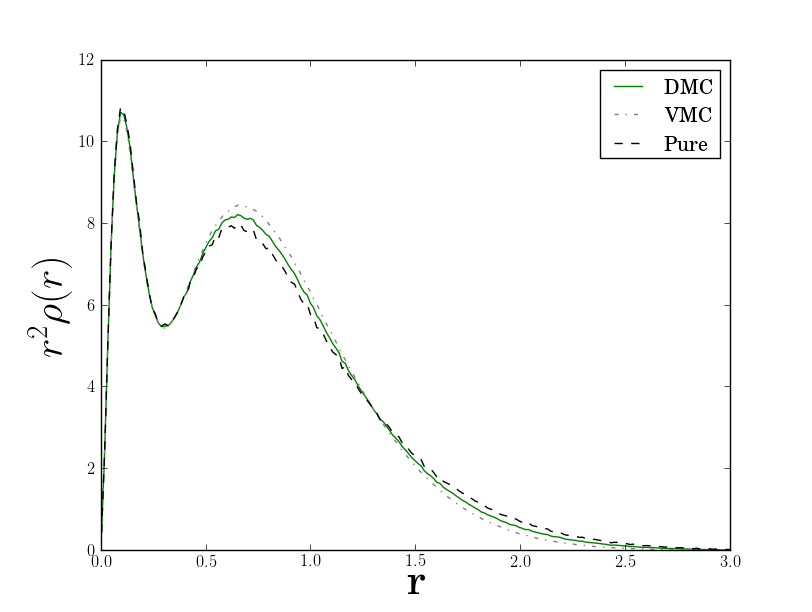
\includegraphics[scale=0.3]{../Graphics/OBD/OBD_Atoms/2D/Neon.png}}  \\
   \subfigure{\includegraphics[scale=0.4]{../Graphics/OBD/OBD_Atoms/3D/Argon.png}} 
   \subfigure{\includegraphics[scale=0.3]{../Graphics/OBD/OBD_Atoms/2D/Argon.png}}  \\
   \subfigure{\includegraphics[scale=0.4]{../Graphics/OBD/OBD_Atoms/3D/Krypton.png}} 
   \subfigure{\includegraphics[scale=0.3]{../Graphics/OBD/OBD_Atoms/2D/Krypton.png}}  \\
  \caption{One-body densities for noble gases. Counting top to bottom: Helium, neon, argon and krypton. A quarter of the spherical density is removed to present a better view of the core. Red and blue color indicate a low and high electron density, respectively. Notice that the radial one-body densities in the right column are multiplied by the radius squared. This is done in order to reveal the characteristics behind a density which otherwise is a generic peak around the origin.}
  \label{fig:OBD_noble_Atoms_2D_combo}
 \end{center}
\end{figure}
 
 

\clearpage
\section{Homonuclear Diatomic Molecules}

The focus regarding homonuclear diatomic molecules, from here on referred to as molecules, has been similar to the focus on atoms, with the exception of parameterizing atomic force fields which can be applied in molecular dynamics simulations. The implementation of molecular systems was achieved by adding $\sim 200$ lines of code. This fact by itself represents a successful result regarding the code structure. As for atoms, the optimal calculations are referred to as experimental results. Details regarding the transformation from atomic to molecular systems are given in Section \ref{sec:homoMolecules}.

\subsection{Ground State Energies}
 
\begin{table}
\begin{center}
\begin{tabular}{lrccrlrrc}
Molecule & $R$ & & \qquad & $E_\mathrm{VMC}$ & & \qquad $E_\mathrm{DMC}$ & \qquad\,\, Expt. & \qquad $\epsilon_\mathrm{rel}$\\
\hline\hline
\ \\
$\mathrm{H_2}$ & 1.4   & &\qquad & -1.1551(3)    & \qquad   & -1.1745(3)   & \qquad $-1.1746$      & \qquad $8.51\cdot 10^{-5}$ \\
\ \\
$\mathrm{Li_2}$& 5.051 & &\qquad & -14.743(3)    & \qquad   & -14.988(2)   & \qquad $-14.99544$    & \qquad $4.96\cdot 10^{-4}$ \\
\ \\
$\mathrm{Be_2}$& 4.63  & &\qquad & -28.666(5)    & \qquad   & -29.301(5)   & \qquad $-29.33854(5)$ & \qquad $1.28\cdot 10^{-3}$  \\
\ \\
$\mathrm{B_2}$ & 3.005 & &\qquad & -47.746(7)    & \qquad   & -49.155(5)   & \qquad $-49.4184$     & \qquad $5.33\cdot 10^{-3}$  \\
\ \\
$\mathrm{C_2}$ & 2.3481& &\qquad & -72.590(8)    & \qquad   & -74.95(1)    & \qquad $-75.923(5)$   & \qquad $1.28\cdot 10^{-2}$  \\
\ \\
$\mathrm{N_2}$ & 2.068 & &\qquad & -102.78(1)    & \qquad   & -106.05(2)   & \qquad $-109.5423$    & \qquad $3.19\cdot 10^{-2}$  \\
\ \\
$\mathrm{O_2}$ & 2.282 & &\qquad & -143.97(2)    & \qquad   & -148.53(2)   & \qquad $-150.3268$    & \qquad $1.2\cdot 10^{-2}$  \\
\ \\
\end{tabular}
\caption{Ground state energies for homonuclear diatomic molecules calculated using VMC and DMC. The distance between the atoms $R$ are taken from Ref. \cite{H_He_exact} for $\mathrm{H_2}$ and from Ref. \cite{UmrigarMolecules} for $\mathrm{Li_2}$ to $\mathrm{O_2}$. The experimental energies, that is, the best possible results available, are taken from Ref. \cite{H_He_exact} for $\mathrm{H_2}$ and from Ref. \cite{ExactMolecules} for $\mathrm{Li_2}$ to $\mathrm{O_2}$. As expected DMC is closer to the experimental energy than VMC. Moreover, the relative error $\epsilon_\mathrm{rel} = |E_\mathrm{DMC} - \mathrm{Expt.}|/|\mathrm{Expt.}|$ is as expected lowest in the case of $\mathrm{H_2}$, and increases with atomic number.}
\label{tab:MoleculesRes}
\end{center}
\end{table}

Table \ref{tab:MoleculesRes} lists the VMC and DMC results with the corresponding experimental energies for $\mathrm{H_2}$ through $\mathrm{O_2}$. As expected, the two-particle result is very close to the experimental value with the same precision as the result for the helium atom in Table \ref{tab:AtomsRes}. The relative error from the experimental energy increases with atomic number, and is far higher than the errors in the case of pure atoms. This comes as a result of the trial wave function being less optimal due to the fact that it does not account for the atomic nuclei interaction term in the molecular Hamiltonian. Nevertheless, taking the simple nature of the trial wave function into consideration, the calculated energies are satisfyingly close to the experimental ones. 

As with atoms, the energies were calculated on a single node, resulting in a rather big statistical error in DMC. Doing the calculations on a supercomputer with an increase in the number of walkers should decrease the errors.

\subsection{One-body densities}

Figure \ref{fig:OBD_Molecules} presents the one-body densities of $\mathrm{Li_2}$, $\mathrm{Be_2}$ and $\mathrm{O_2}$. The densities have strong peaks located at a distance equal to half of the listed core separation $R$, indicating that the atomic nuclei interaction still dominates the general shape of the distributions. Moreover, it is clear by looking at the figure that most of the electrons are on the side facing the opposite nucleus, leading to the conclusion that the molecules share a covalent bond \cite{UniversityPhysics}. This is especially clear in the case of the oxygen molecule, where there is a small formation of electrons on the inner side of the nuclei.

\vspace{2cm}
\renewcommand\floatpagefraction{.9}
\begin{figure}[h]
 \begin{center}
   \subfigure{\includegraphics[scale=0.4]{../Graphics/OBD/OBD_MOL/Li2_3D.png}} 
   \subfigure{\includegraphics[scale=0.3]{../Graphics/OBD/OBD_MOL/Li2_2D.png}}  \\
   \subfigure{\includegraphics[scale=0.4]{../Graphics/OBD/OBD_MOL/Be2_3D.png}} 
   \subfigure{\includegraphics[scale=0.3]{../Graphics/OBD/OBD_MOL/Be2_2D.png}}  \\
   \subfigure{\includegraphics[scale=0.4]{../Graphics/OBD/OBD_MOL/O2_3D.png}} 
   \subfigure{\includegraphics[scale=0.3]{../Graphics/OBD/OBD_MOL/O2_2D.png}}
  \caption{One-body densities of $\mathrm{Li_2}$ (top), $\mathrm{Be_2}$ (middle) and $\mathrm{O_2}$ (bottom). The figures to the left are spherical densities sliced through the middle to better reveal the core structure. The figures to the right are radial one-body densities projected on the nucleus-nucleus axis. Red and blue color indicate a high and low electron density, respectively. The right-hand figures are symmetric around the origin.}
  \label{fig:OBD_Molecules}
 \end{center}
\end{figure}
\renewcommand\floatpagefraction{.7}

\clearpage
\subsection{Parameterizing Force Fields}

\begin{figure}
 \begin{center}
  \subfigure[$\mathrm{H_2}$]{\includegraphics[scale=0.37]{../Graphics/R_VS_E/R_vs_E_hyd_pure.png}}
  \subfigure[$\mathrm{Li_2}$]{\includegraphics[scale=0.37]{../Graphics/R_VS_E/R_vs_E_lit_pure.png}} 
  \caption{Top figures: The distance between the atoms $R$ vs. the potential and total energy calculated using QMC. To the left: $\mathrm{H_2}$. To the right: $\mathrm{Li_2}$. It is evident that there exists a well-defined energy minimum in the case of hydrogen. For lithium this is not the case, which is expected since lithium does not appear naturally in a diatomic gas phase, but rather as an ionic compound in other molecules \cite{UniversityPhysics}. Bottom figure: The general shape of the Lennard-Jones potential commonly used in molecular dynamics simulations as an approximation to the potential between atoms. The top figures clearly resemble the Lennard-Jones 12-6 potential, leading to the conclusion that QMC calculations can be used to parameterize a more realistic potential.}
  \label{fig:molecules_R_vs_E}
  \setcounter{subfigure}{2}
  \subfigure[The Lennard-Jones 12-6 potential with $\sigma=\epsilon=1$.]{\includegraphics[scale=0.5]{../Graphics/R_VS_E/LD.png}}
  \label{fig:LennardJones}
 \end{center}
\end{figure}

In molecular dynamics, it is custom to use the \textit{Lennard Jones 12-6 potential} as an ansatz to the interaction between pairs of atoms \cite{MD1, MD2}

\begin{equation}
 V(R) = 4\epsilon \left(\left(\frac{\sigma}{R}\right)^{12} - \left(\frac{\sigma}{R}\right)^{6}\right),
\end{equation}

where $\epsilon$ and $\sigma$ are parameters which can be fit to a given system.

However, the force field can be parameterized in greater detail using QMC calculations, resulting in a more precise molecular dynamics simulation \cite{forcesQMC}. The quantity of interest is the \textit{force}, that is, the gradient of the potential. The classical potential in molecular dynamics does not correspond to the potential in the Schrödinger equation, due to the fact that the kinetic energy contribution from the electrons is not counted as part of the total kinetic energy in the molecular dynamics simulation. Hence it is the total energy of the Schrödinger equation which corresponds to the potential energy in molecular dynamics. In the case of diatomic molecules this means that 

\begin{equation}
 F_\mathrm{MD} = \frac{\mathrm{d}\langle E \rangle}{\mathrm{d}R}.
\end{equation}

Expressions for this derivative can be obtained in ab-initio methods by using the Hellmann-Feynman theorem \cite{forcesQMC}. However, the derivative can be approximated by the slope of the energy in Figure \ref{fig:molecules_R_vs_E}. The figure shows that there are clear similarities between the widely used Lennard-Jones 12-6 potential and the results of QMC calculations done in this thesis, leading to the conclusion that the current state of the code can in fact produce approximations to atomic force fields for use in molecular dynamics.

For more complicated molecules, modelling the force using a single parameter $R$ does not serve as a good approximation. However, the force can be found as a function of several angles, radii, etc., which in turn can be used to parameterize a more complicated molecular dynamics potential. An example of such a potential is the \textit{ReaxFF} potential for hydrocarbons \cite{ReaxFF}.






 
 

 
 
 



